%%%%%%%%%%%%%%%%%%%%%%%%%%%%%%%%%%%%%%%%%%%%%%%%%%%%%%%%%%%%%%%%%%%%
%%
%%                     AFD
%%
%%%%%%%%%%%%%%%%%%%%%%%%%%%%%%%%%%%%%%%%%%%%%%%%%%%%%%%%%%%%%%%%%%%%

\begin{frame}{Definição do movimento de barra fixa}
    \begin{itemize}
        \item A \textbf{barra} fixa é instalada a uma altura tal, que o avaliado, mantendo-se pendurado, com os cotovelos em extensão, não tenha contato dos pés com o solo;
        \item  A posição da \textbf{pegada} é pronada (dorso da mão voltado para o rosto) e a abertura das mãos corresponde à distância biacromial (largura dos ombros); 
        \item  Após assumir essa posição, o avaliado deverá elevar o corpo até que o \textbf{queixo ultrapasse o nível da barra}, após o que retornará à posição inicial; 
        \item  O movimento é \textbf{repetido} tantas vezes quanto possível, sem limite de tempo. 
    \end{itemize}
\end{frame}

\begin{frame}{Definição do movimento de barra fixa}
    \begin{itemize}
        \item  Os cotovelos deverão estar em \textbf{extensão} total para o início de flexão; 
        \item  É permitido \textbf{repouso} entre um movimento e outro, contudo, o avaliado não poderá tocar os pés no solo; 
        \item  \textbf{Não são permitidos} movimentos de quadris ou pernas e extensão da coluna cervical como formas de auxiliar na execução da prova. 
        \item  A não extensão total dos cotovelos antes do início de nova execução é considerado um \textbf{movimento incorreto}, o qual não será computado no desempenho do candidato. 
        \item  Somente é contado o número de movimentos completados corretamente.
    \end{itemize}
\end{frame}


\begin{frame}{Estratégia para detecção do movimento correto de barra fixa}

    \begin{figure}[!ht]
    \centering
    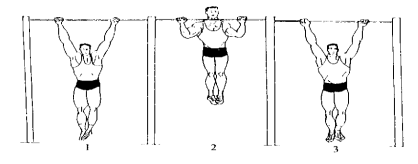
\includegraphics[scale=0.5]{img/desenvolvimento/barraFixa/barraFixa.jpg}
    \caption*{Fonte - (GOIÁS, 2017)}
    \end{figure}

    
    \begin{enumerate}
        \item  A primeira etapa engloba a posição inicial.

        \item  A segunda etapa engloba a fase de contração concêntrica, onde o indivíduo eleva seu corpo até que seu queixo ultrapasse o nível da barra.

        \item  A terceira etapa engloba a fase de contração excêntrica.
    \end{enumerate}
\end{frame}


\begin{frame}{Computação do movimento barra fixa}

    \begin{figure}[!ht]
    \centering
    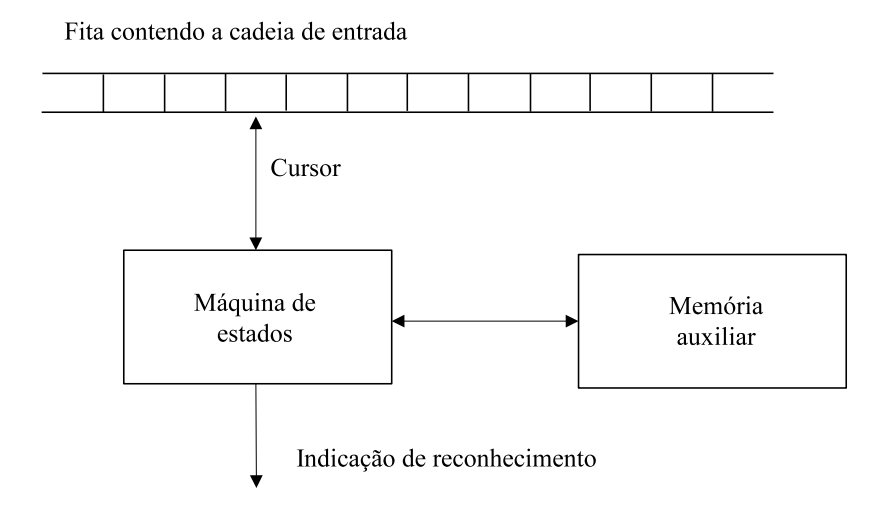
\includegraphics[scale=1.3]{img/desenvolvimento/estrategia/reconhecedor.png}
    \caption*{Fonte - (OLIVETE, 2020).}
    \end{figure}
    
\end{frame}


\begin{frame}{Composição do alfabeto}
    
    O AFD construído opera em relação a um alfabeto específico. Esse alfabeto é constituído por características extraídas de cada \textit{frame}. Cada símbolo do alfabeto é representado por uma 4-upla de características (A,B,C,D)
    
    \begin{itemize}
        \item[A] - Presença das mãos na barra.
        \item[B] - Ocorrência da extensão dos cotovelos.
        \item[C] - Ocorrência da ultrapassagem do queixo sobre a barra.
        \item[D] - Existência de movimento nos quadris.
    \end{itemize} 

\end{frame}



\begin{frame}{Alfabeto}
    \[
    \begin{aligned}
    \Sigma = \{ &(0, 0, 0, 0), (0, 0, 0, 1), (0, 0, 1, 0), (0, 0, 1, 1), \\
                &(0, 1, 0, 0), (0, 1, 0, 1), (0, 1, 1, 0), (0, 1, 1, 1), \\
                &(1, 0, 0, 0), (1, 0, 0, 1), (1, 0, 1, 0), (1, 0, 1, 1), \\
                &(1, 1, 0, 0), (1, 1, 0, 1), (1, 1, 1, 0), (1, 1, 1, 1) \}
    \end{aligned}
    \]
\end{frame}


\begin{frame}{Estados}
    O AFD desenvolvido consiste em um conjunto de sete estados:\\
    \vspace{0.8cm}
    $Q$ = \{Preparação, Início, Concêntrica, Meta, Excêntrica, Erro, Fim\}
     
\end{frame}



\begin{frame}{Diagrama de Estados}

    \begin{figure}[!ht]
    \centering
    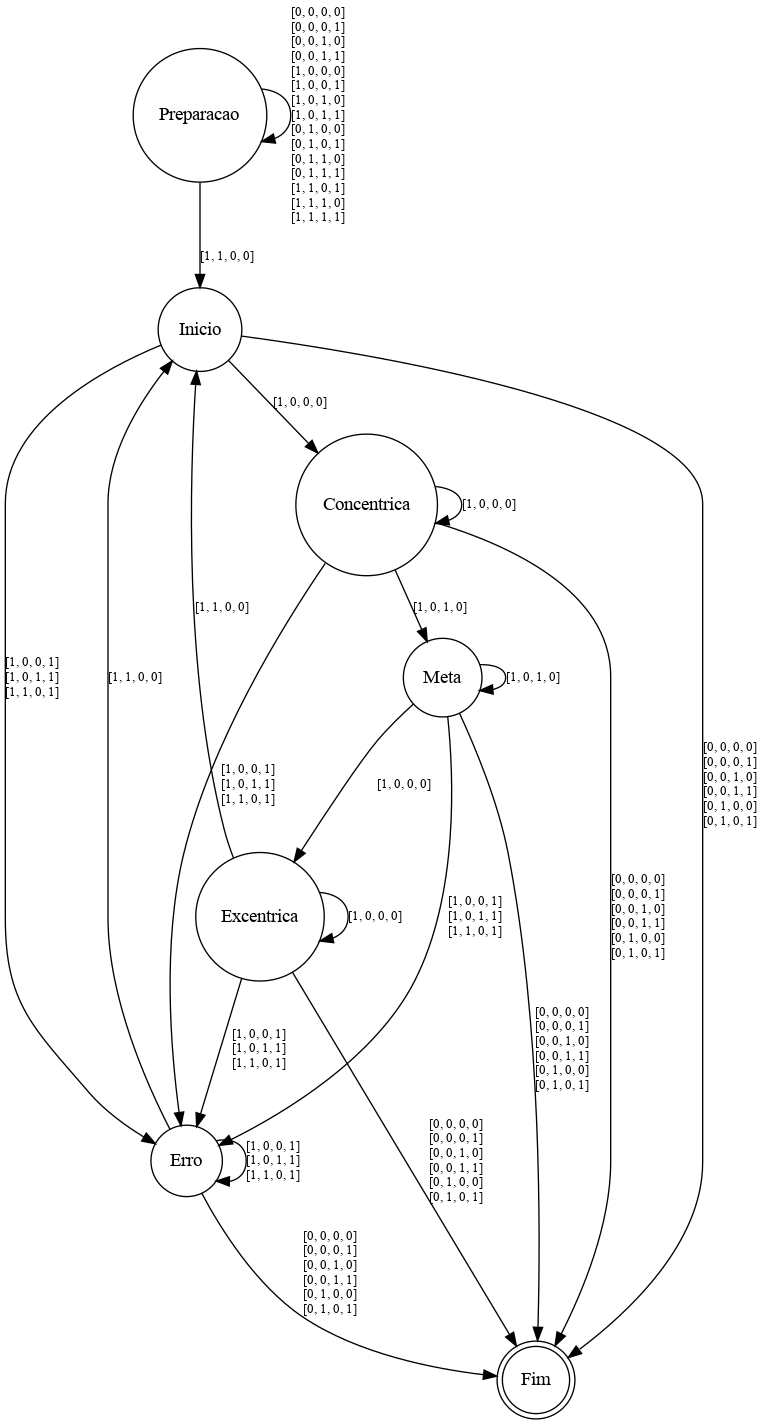
\includegraphics[scale=0.13]{img/desenvolvimento/estrategia/afd_barra.png}
    \caption*{Fonte - Proprio autor 2023.}
    \end{figure}
    
\end{frame}


%%%%%%%%%%%%%%%%%%%%%%%%%%%%%%%%%%%%%%%%%%%%%%%%%%%%%%%%%%%%%%%%%%%%
%%
%%                     Processos
%%
%%%%%%%%%%%%%%%%%%%%%%%%%%%%%%%%%%%%%%%%%%%%%%%%%%%%%%%%%%%%%%%%%%%%


\begin{frame}{Extração de informação frame a frame}
    \begin{itemize}
        \item  Detecção da barra 
        \item  Inclinação da barra
        \item  Reconhecimento de pose humana 
        \item  Mão na barra 
        \item  Braço esticado
        \item  Ultrapassagem do queixo a barra
        \item  Movimentação do quadril
    \end{itemize}
\end{frame}






%%%%%%%%%%%%%%%%%%%%%%%%%%%%%%%%%%%%%%%%%%%%%%%%%%%%%%%%%%%%%%%%%%%%
%%
%%                     Método
%%
%%%%%%%%%%%%%%%%%%%%%%%%%%%%%%%%%%%%%%%%%%%%%%%%%%%%%%%%%%%%%%%%%%%%
%%
%%                     Detecção da barra
%%
%%%%%%%%%%%%%%%%%%%%%%%%%%%%%%%%%%%%%%%%%%%%%%%%%%%%%%%%%%%%%%%%%%%%


\begin{frame}{Detecção da barra - Fluxograma}
    \begin{figure}[!ht]
    \centering
    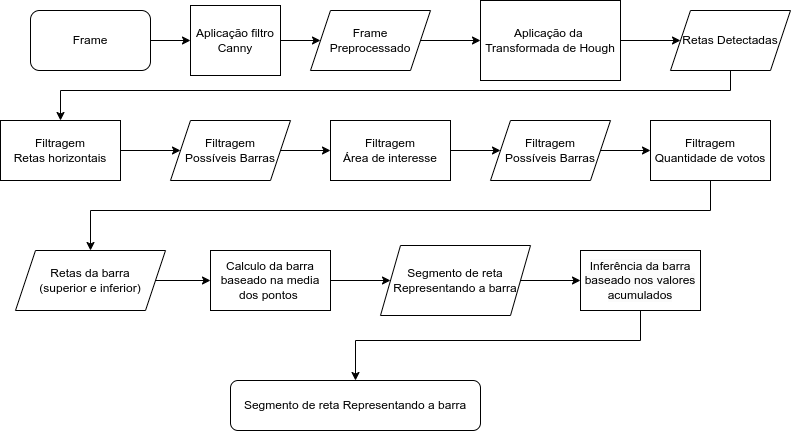
\includegraphics[scale=0.4]{img/desenvolvimento/detectaBarra/fluxograma.png}
    \caption*{Fonte - Próprio Autor.}
    \end{figure}
\end{frame}

\begin{frame}{Detecção da barra - Filtro de Canny.}
    \begin{itemize}
        \item  Redução de ruído         (Gaussiano - Blur)
        \item  Cálculo do Gradiente     (Sobel - detecção de contornos)
        \item  Supressão não máxima     (Filtro Passa Alta) 
        \item  Limite duplo             (minVal e maxVal)
        \item  Limite de histerese      (conectividade)
    \end{itemize}
\end{frame}

\begin{frame}{Detecção da barra - Aplicação do filtro de Canny.}
    \begin{figure}[!ht]
    \centering
    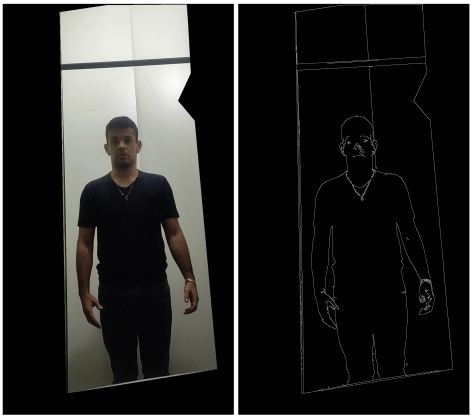
\includegraphics[scale=0.45]{img/desenvolvimento/detectaBarra/canny.png}
    \caption*{Fonte - Próprio Autor.}
    \end{figure}
\end{frame}



\begin{frame}{Detecção da barra - Segmentos de Retas.}
    \begin{figure}[!ht]
    \centering
    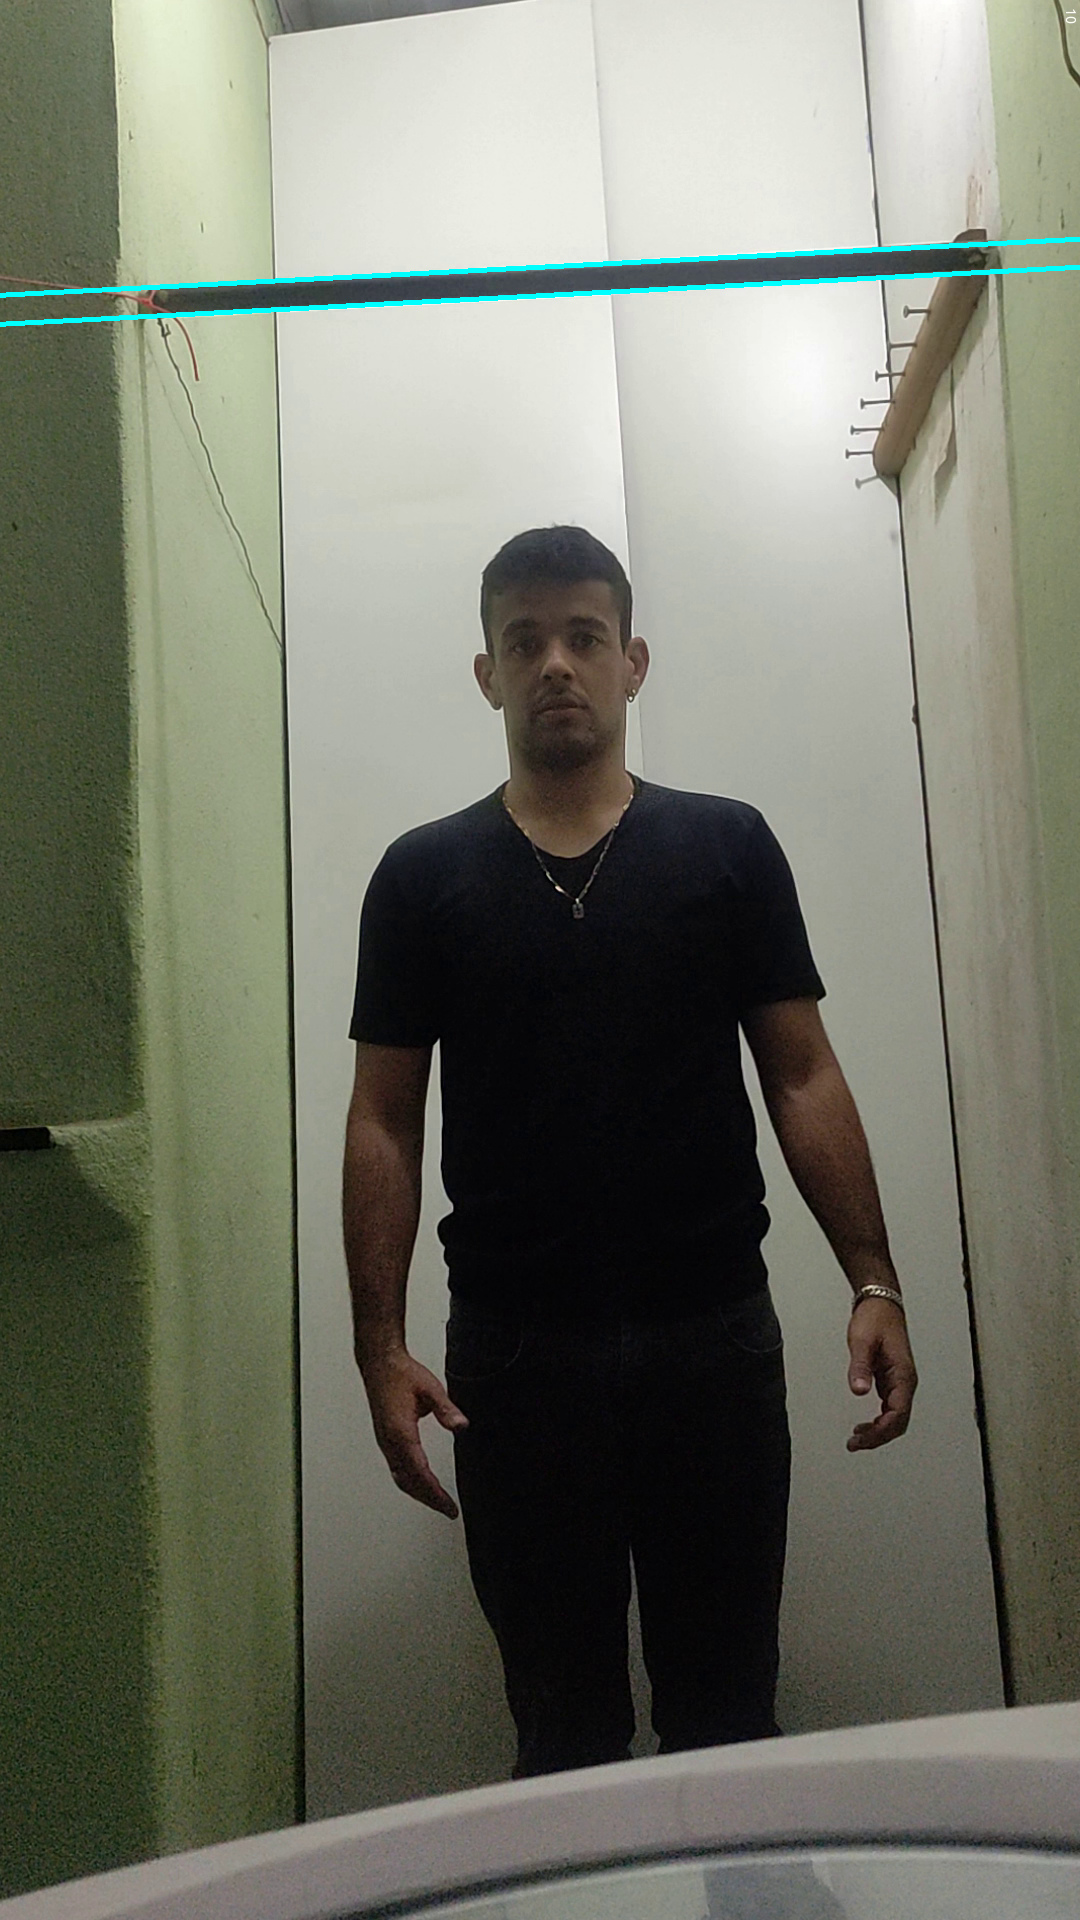
\includegraphics[scale=0.1]{img/desenvolvimento/detectaBarra/barras.png}
    \caption*{Fonte - Próprio Autor.}
    \end{figure}
\end{frame}


\begin{frame}{Detecção da barra - Segmento de Reta Unificado.}
    \begin{figure}[!ht]
    \centering
    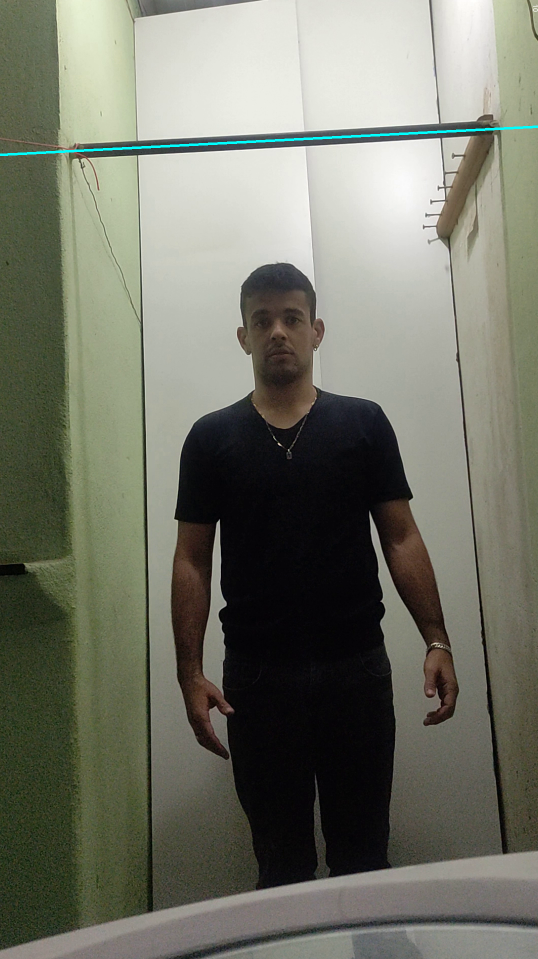
\includegraphics[scale=0.20]{img/desenvolvimento/detectaBarra/barra_unificada.png}
    \caption*{Fonte - Próprio Autor.}
    \end{figure}
\end{frame}

%%%%%%%%%%%%%%%%%%%%%%%%%%%%%%%%%%%%%%%%%%%%%%%%%%%%%%%%%%%%%%%%%%%%
%%
%%                     Inclinação da barra
%%
%%%%%%%%%%%%%%%%%%%%%%%%%%%%%%%%%%%%%%%%%%%%%%%%%%%%%%%%%%%%%%%%%%%%
\begin{frame}{Inclinação da barra}
    \begin{figure}[!ht]
    \centering
    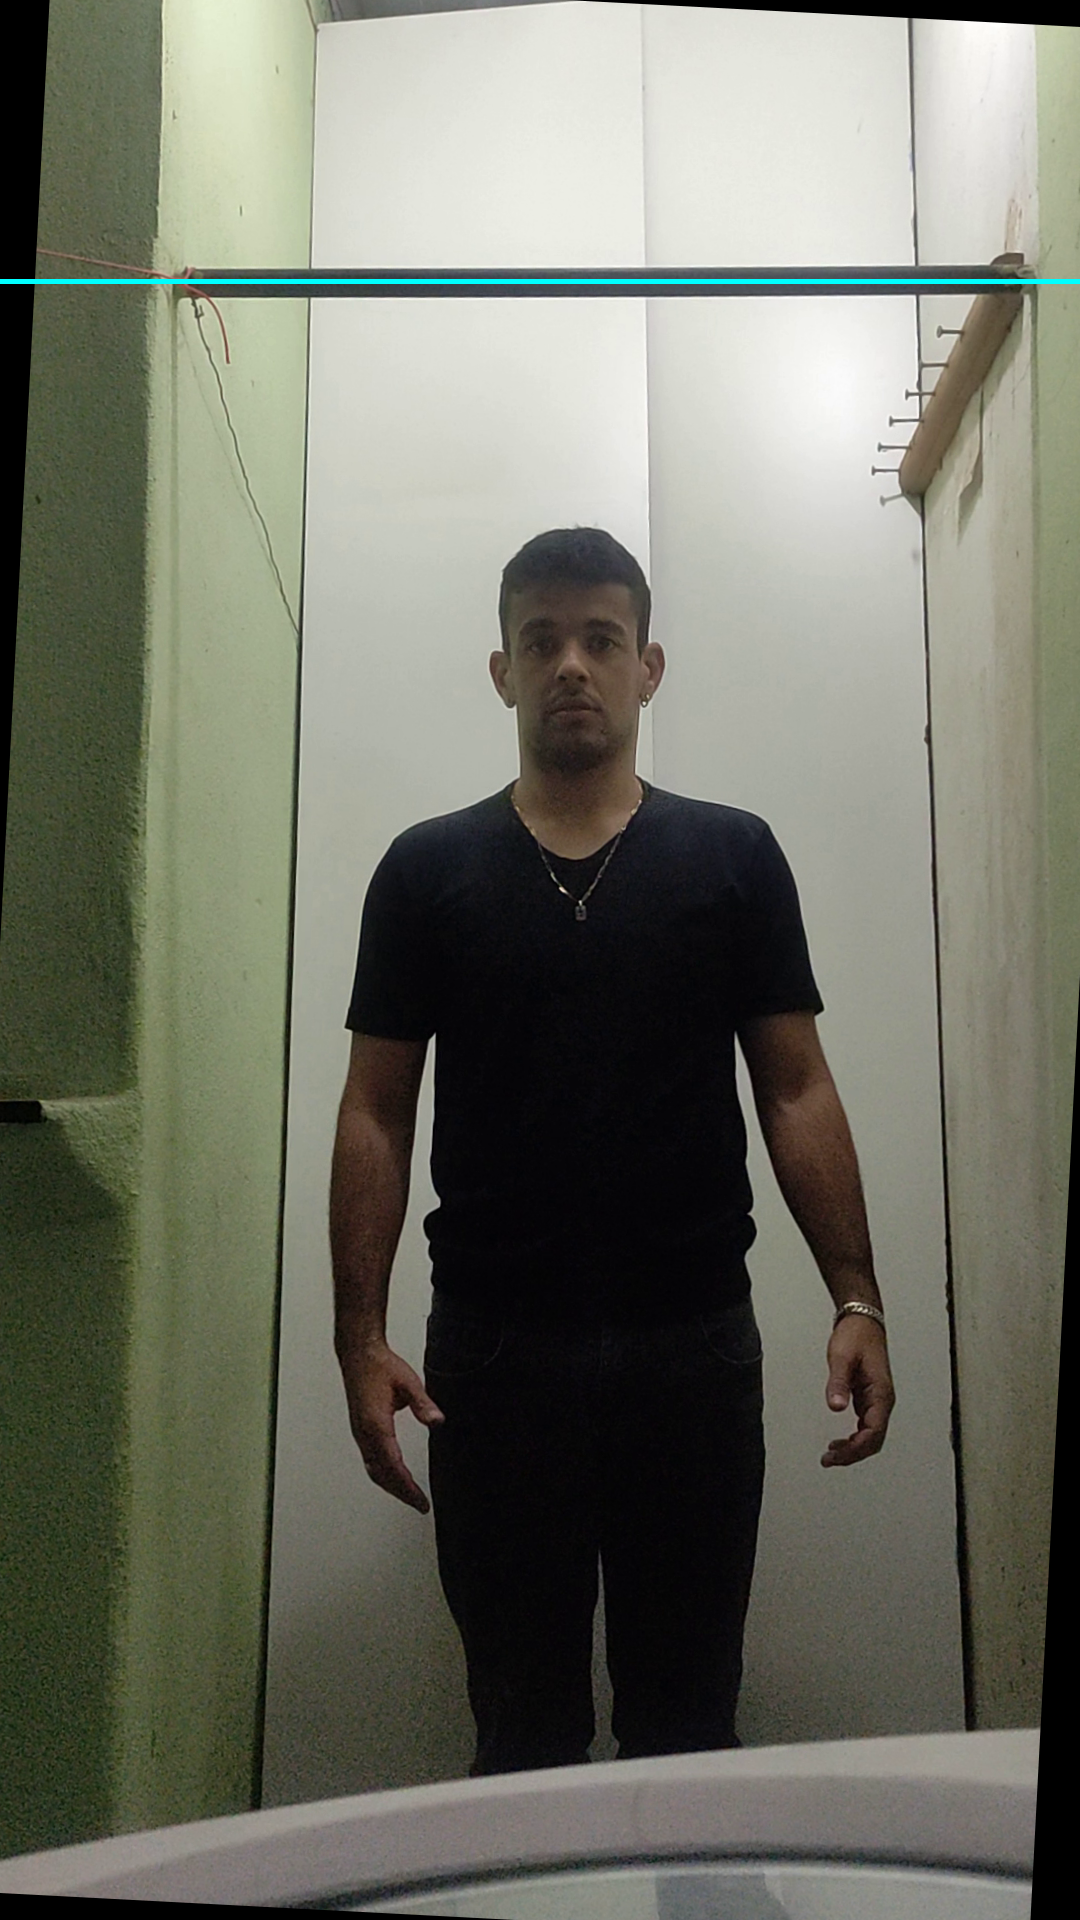
\includegraphics[scale=0.1]{img/desenvolvimento/inclinacaoBarra/barra_rotacionada.png}
    \caption*{Fonte - Próprio Autor.}
    \end{figure}
\end{frame}


%%%%%%%%%%%%%%%%%%%%%%%%%%%%%%%%%%%%%%%%%%%%%%%%%%%%%%%%%%%%%%%%%%%%
%%
%%                     Reconhecimento de pose humana
%%
%%%%%%%%%%%%%%%%%%%%%%%%%%%%%%%%%%%%%%%%%%%%%%%%%%%%%%%%%%%%%%%%%%%%

\begin{frame}{Reconhecimento de pose humana - Pontos chaves}
    \begin{figure}[!ht]
    \centering
    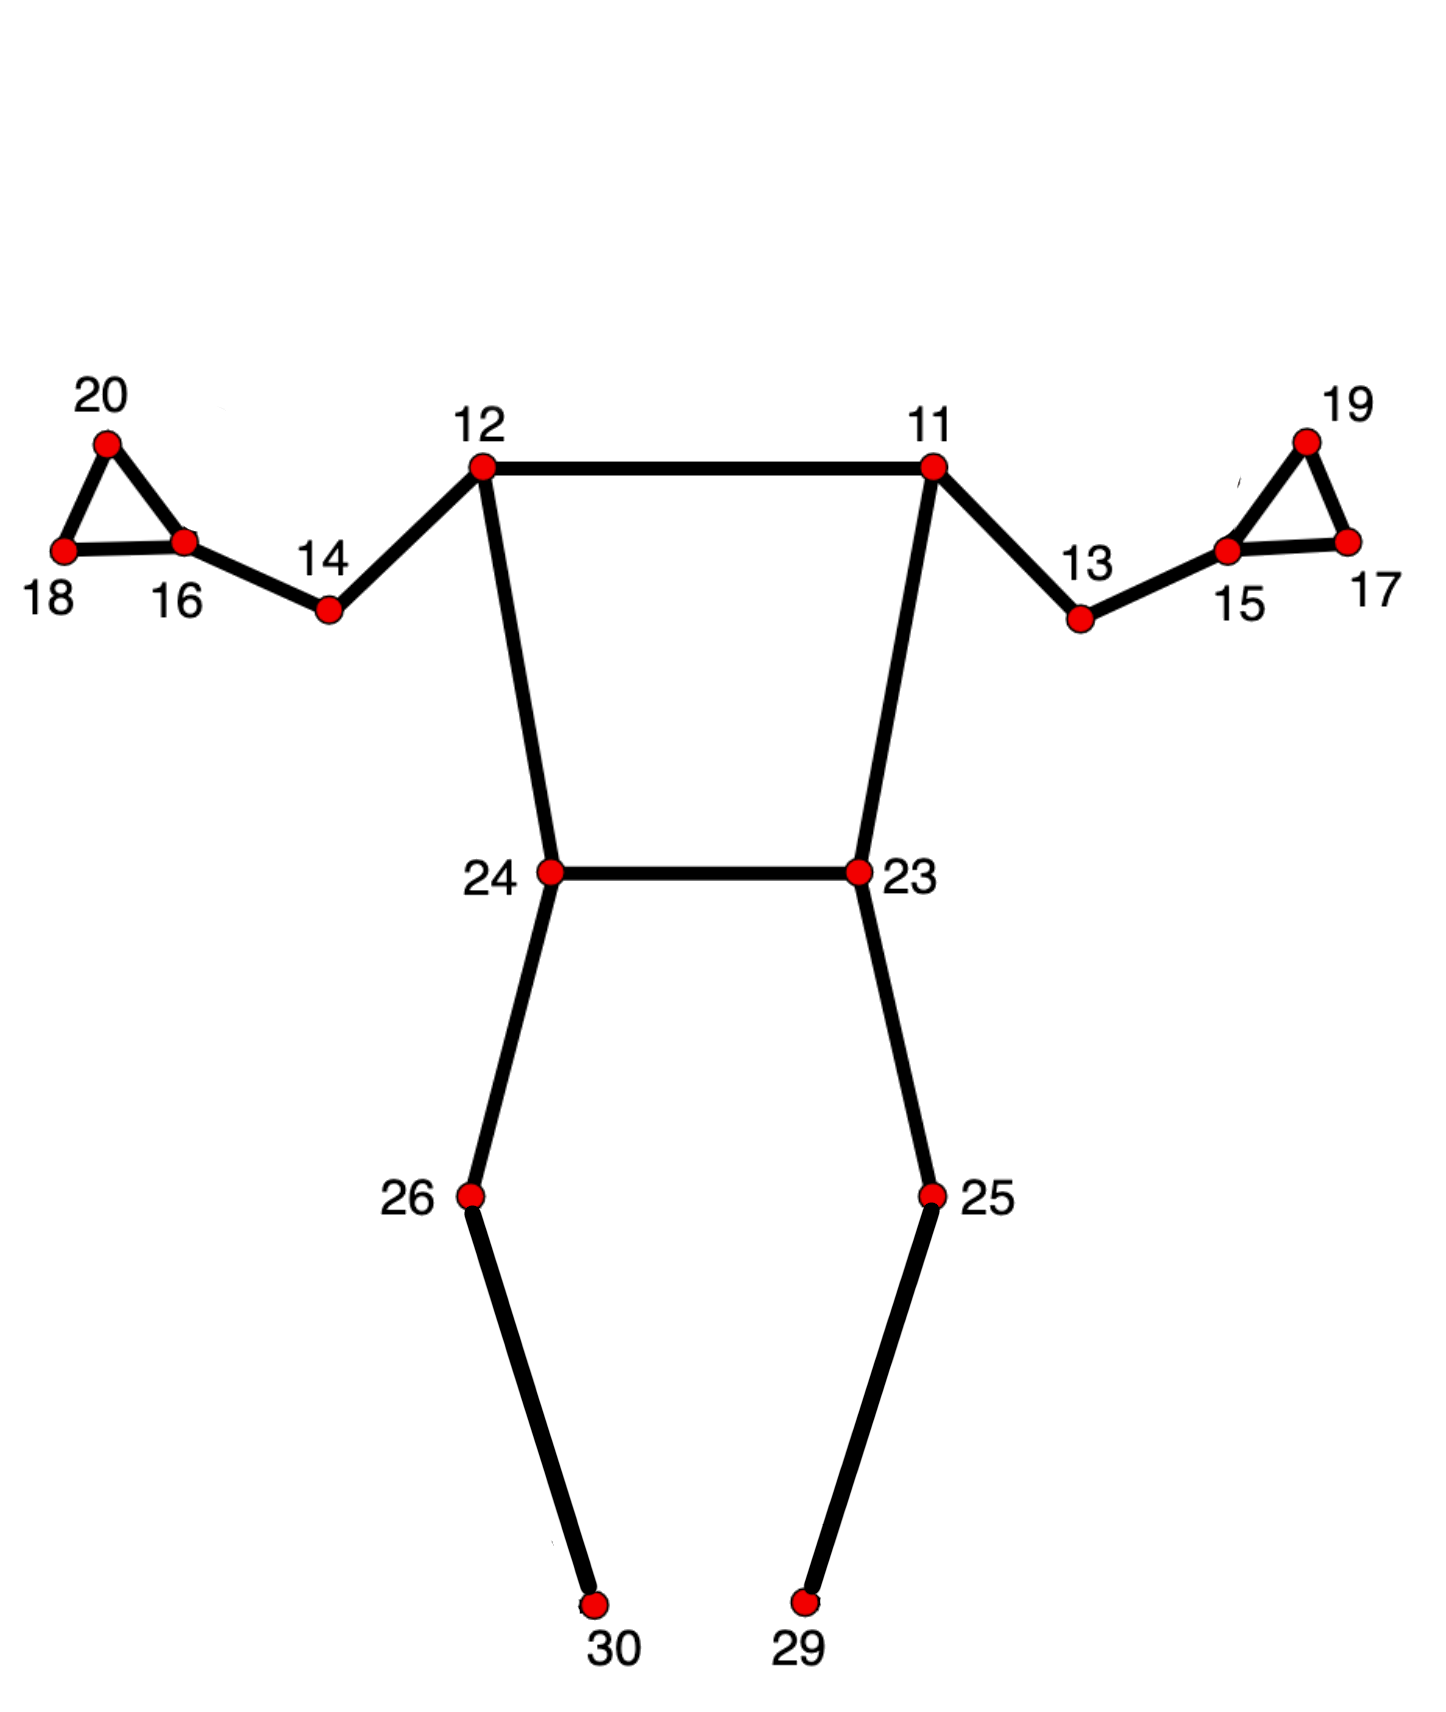
\includegraphics[scale=0.2]{img/desenvolvimento/eph/pose_landmarks_custom.png}
    \caption*{Fonte - Próprio Autor.}
    \end{figure}
\end{frame}

\begin{frame}{Reconhecimento de pose humana }
    \begin{figure}[!ht]
    \centering
    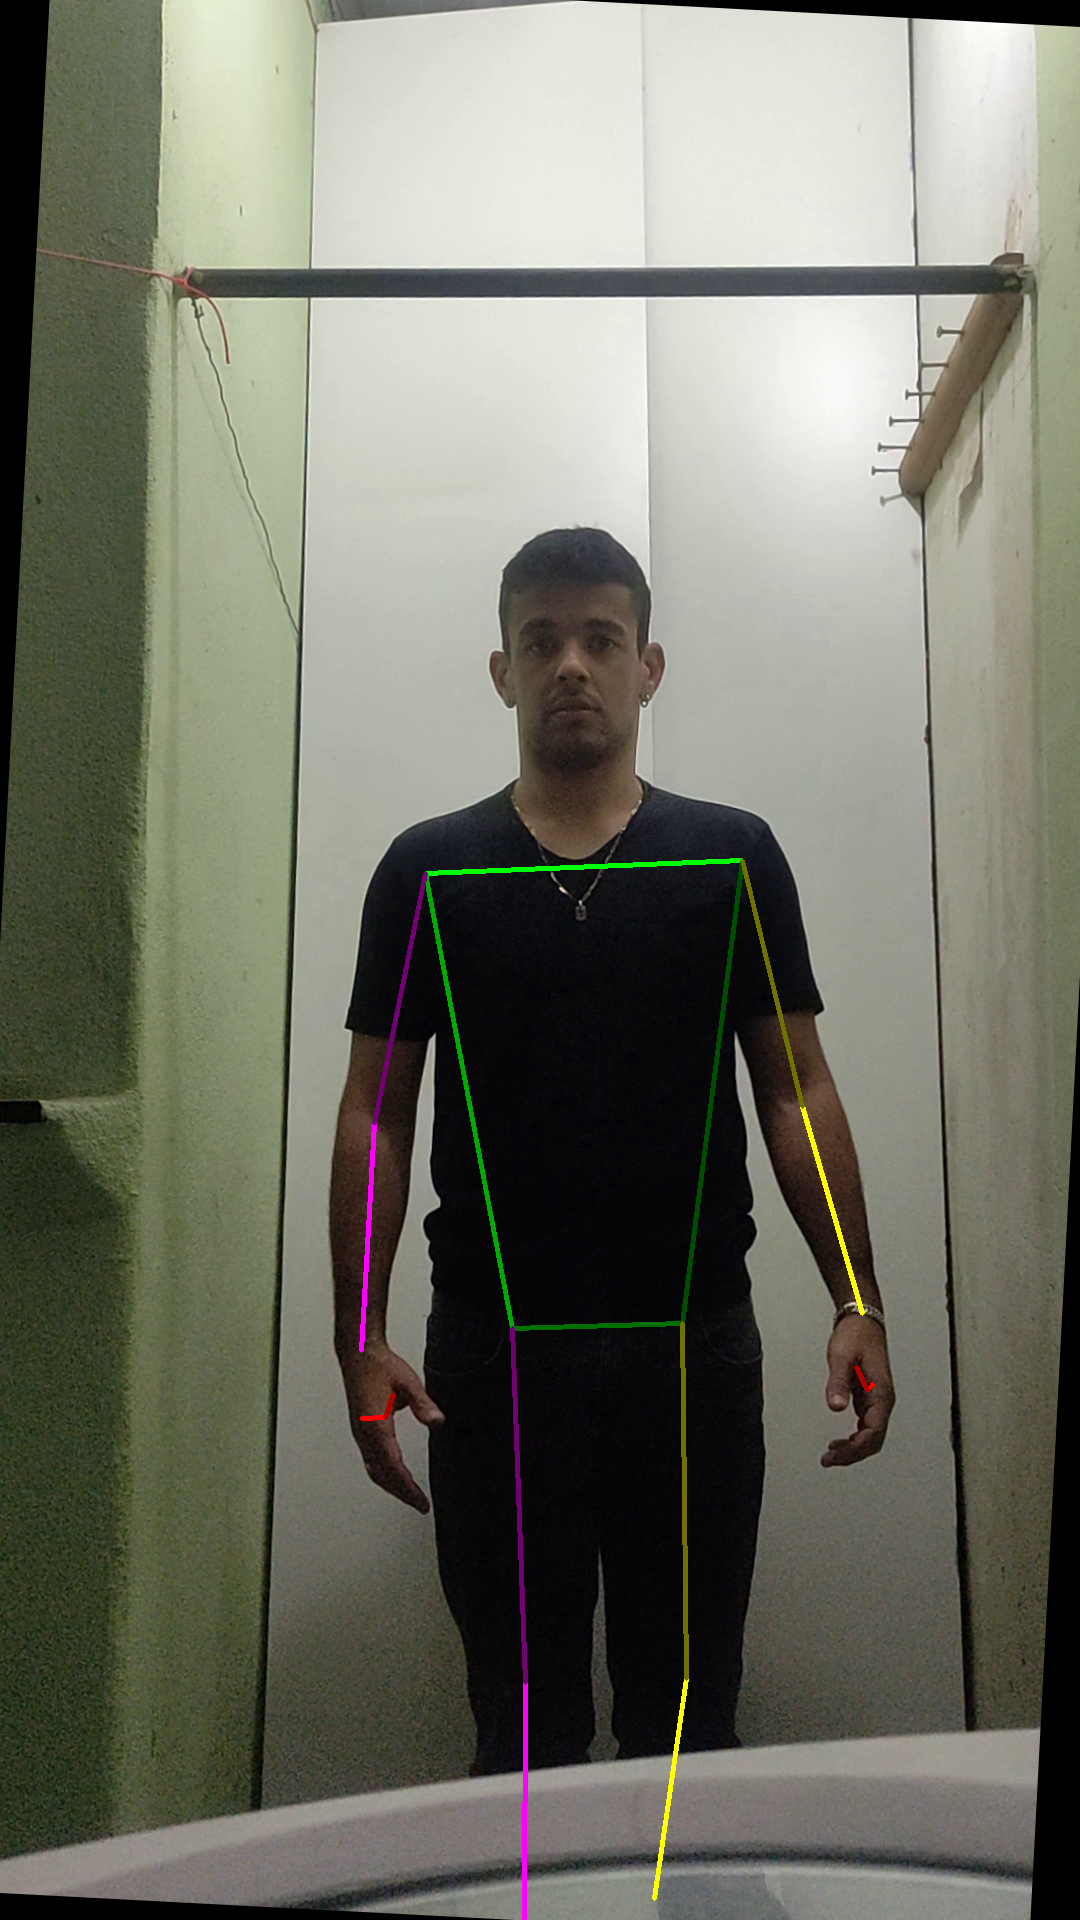
\includegraphics[scale=0.1]{img/desenvolvimento/eph/landmark.png}
    \caption*{Fonte - Próprio Autor.}
    \end{figure}
\end{frame}


%%%%%%%%%%%%%%%%%%%%%%%%%%%%%%%%%%%%%%%%%%%%%%%%%%%%%%%%%%%%%%%%%%%%
%%
%%                     Mão na barra
%%
%%%%%%%%%%%%%%%%%%%%%%%%%%%%%%%%%%%%%%%%%%%%%%%%%%%%%%%%%%%%%%%%%%%%

\begin{frame}{Mão na barra - Fluxograma}
    \begin{figure}[!ht]
    \centering
    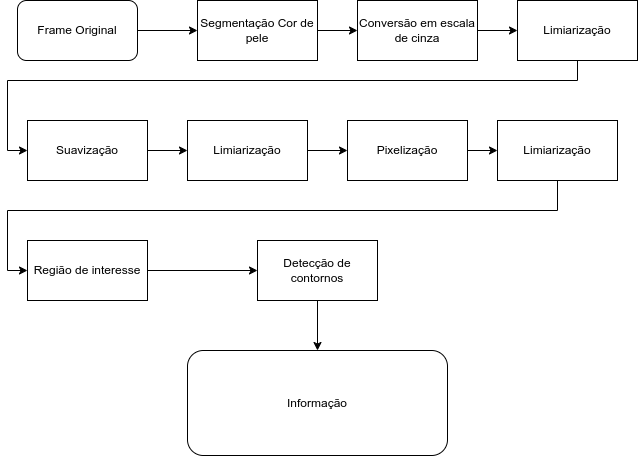
\includegraphics[scale=0.4]{img/desenvolvimento/maoBarra/fluxograma.png}
    \caption*{Fonte - Próprio Autor.}
    \end{figure}
\end{frame}


\begin{frame}{Mão na barra - Imagem original}
    \begin{figure}[!ht]
    \centering
    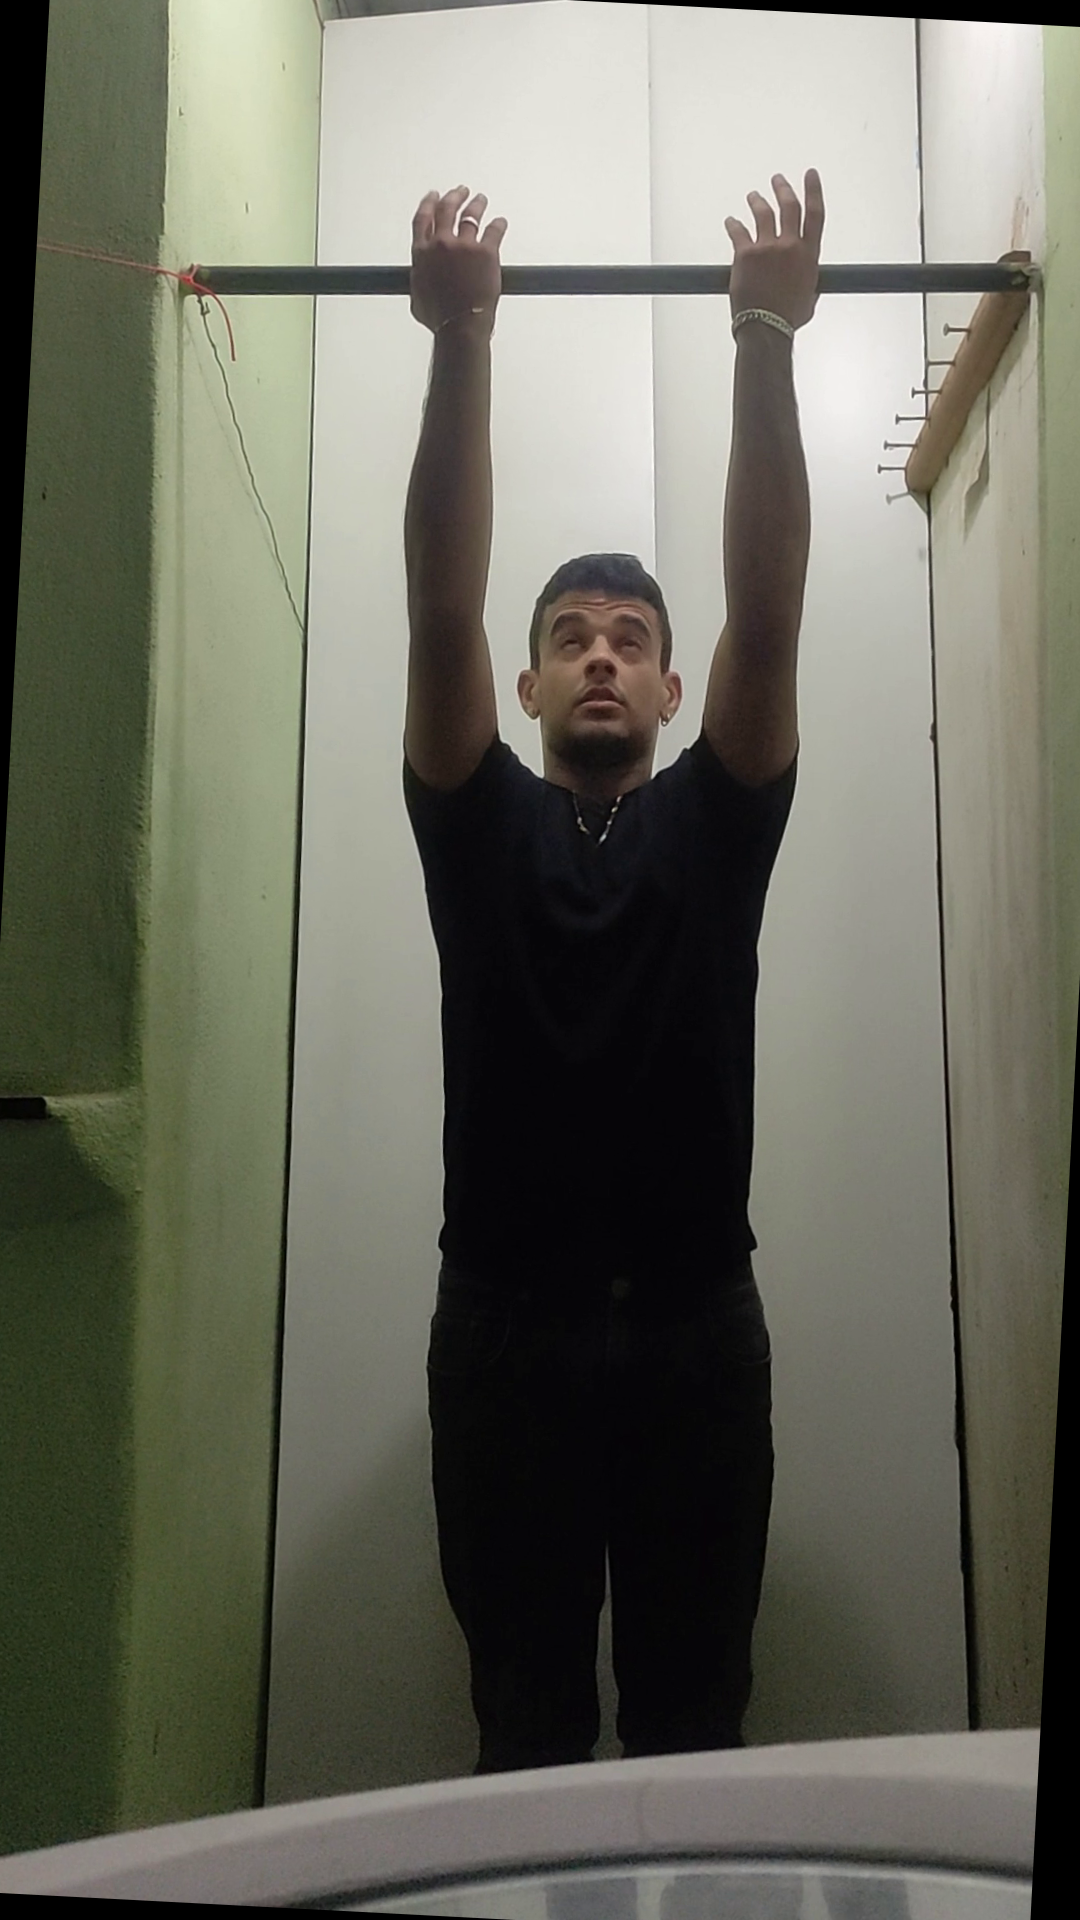
\includegraphics[scale=0.1]{img/desenvolvimento/maoBarra/original.png}
    \caption*{Fonte - Próprio Autor.}
    \end{figure}
\end{frame}


\begin{frame}{Mão na barra - Filtro cor de pele}
    \begin{figure}[!ht]
    \centering
    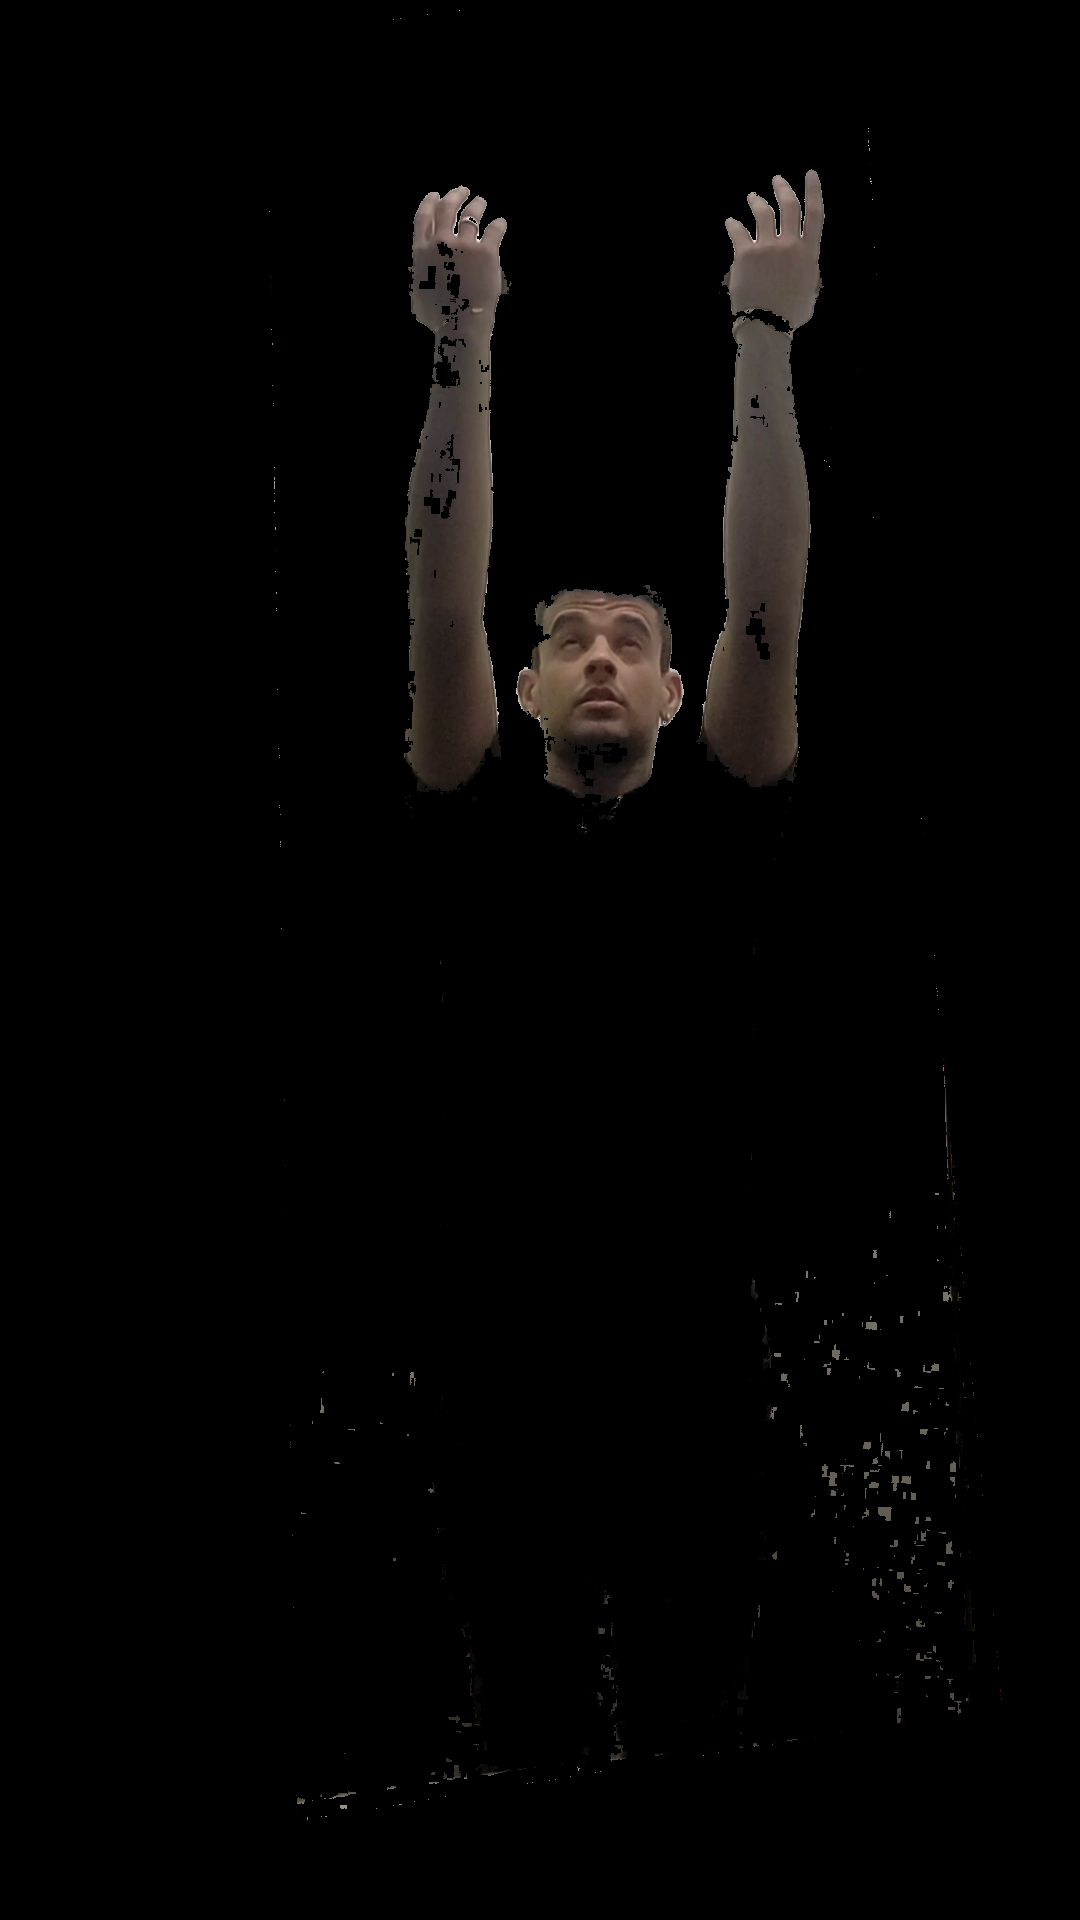
\includegraphics[scale=0.1]{img/desenvolvimento/maoBarra/skin.png}
    \caption*{Fonte - Próprio Autor.}
    \end{figure}
\end{frame}


\begin{frame}{Mão na barra - Escala de cinza}
    \begin{figure}[!ht]
    \centering
    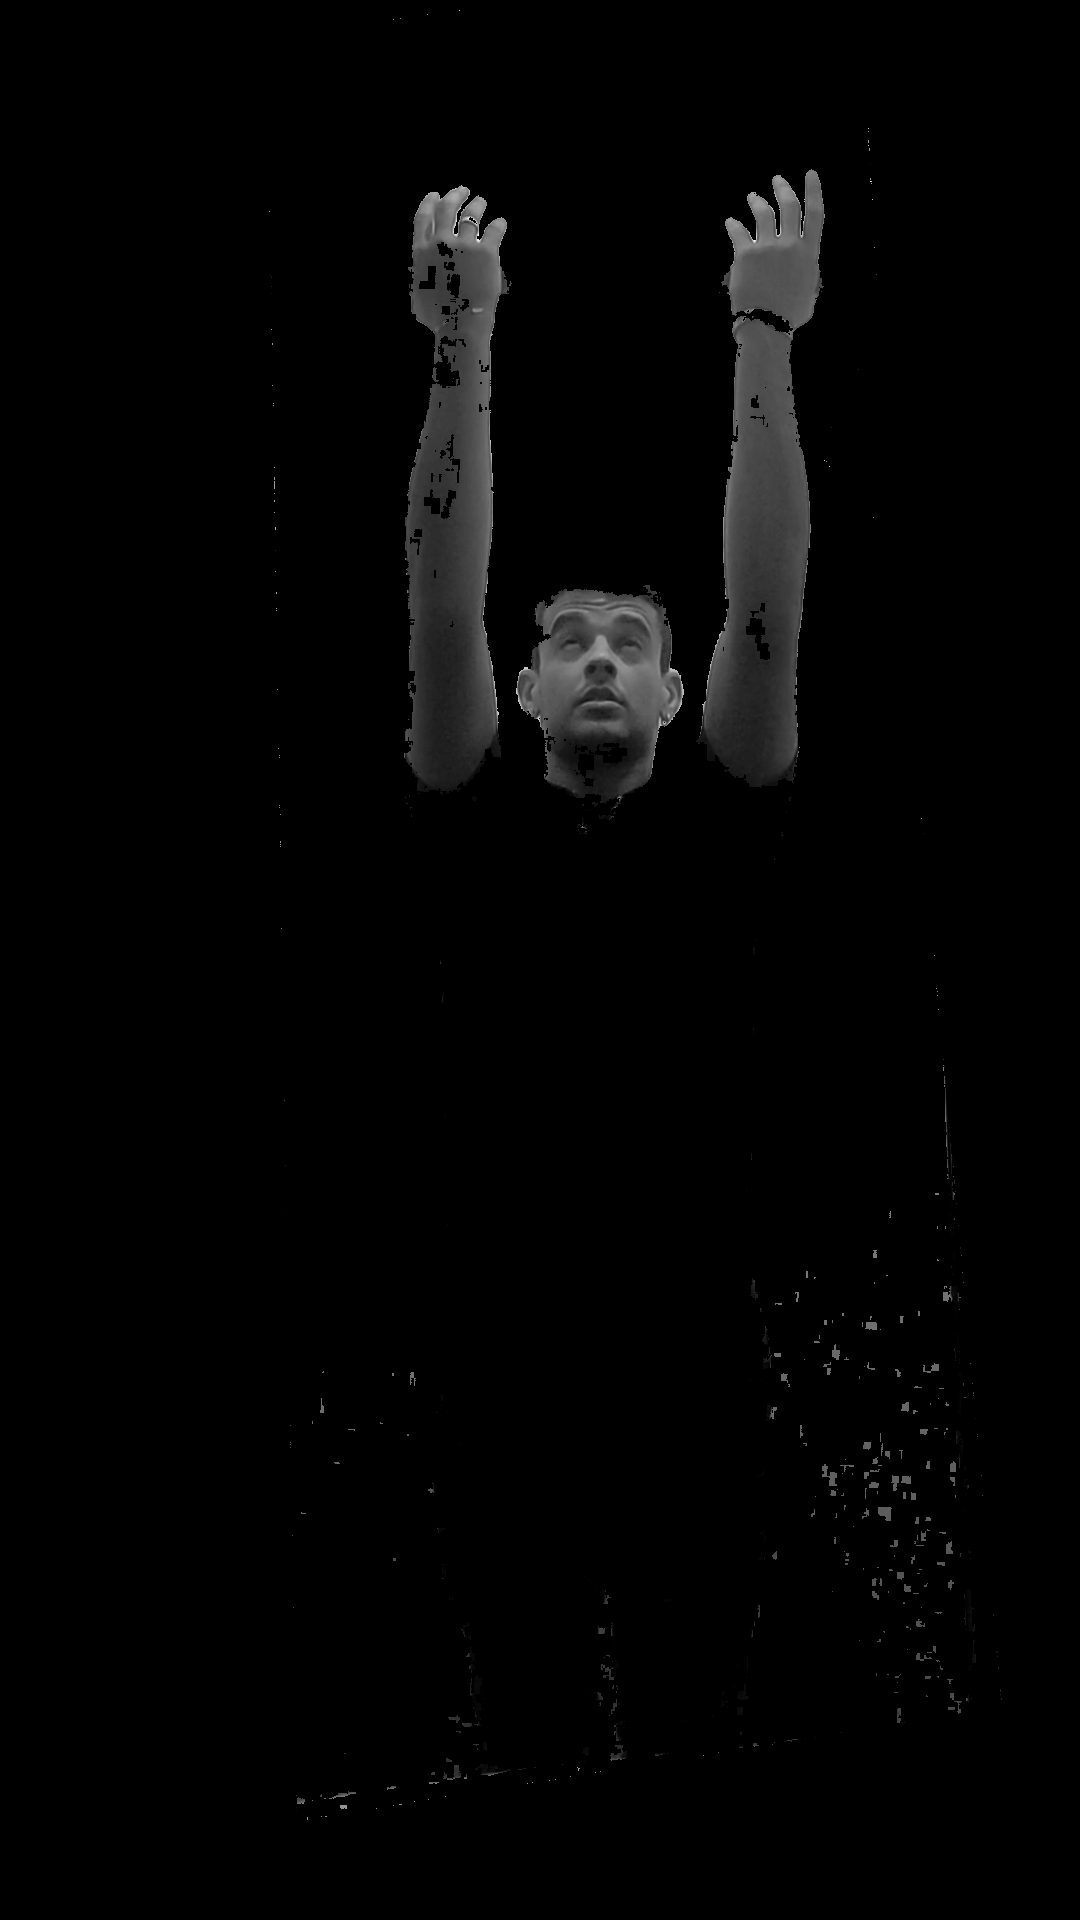
\includegraphics[scale=0.1]{img/desenvolvimento/maoBarra/gray.png}
    \caption*{Fonte - Próprio Autor.}
    \end{figure}
\end{frame}

\begin{frame}{Mão na barra - Limiarização}
    \begin{figure}[!ht]
    \centering
    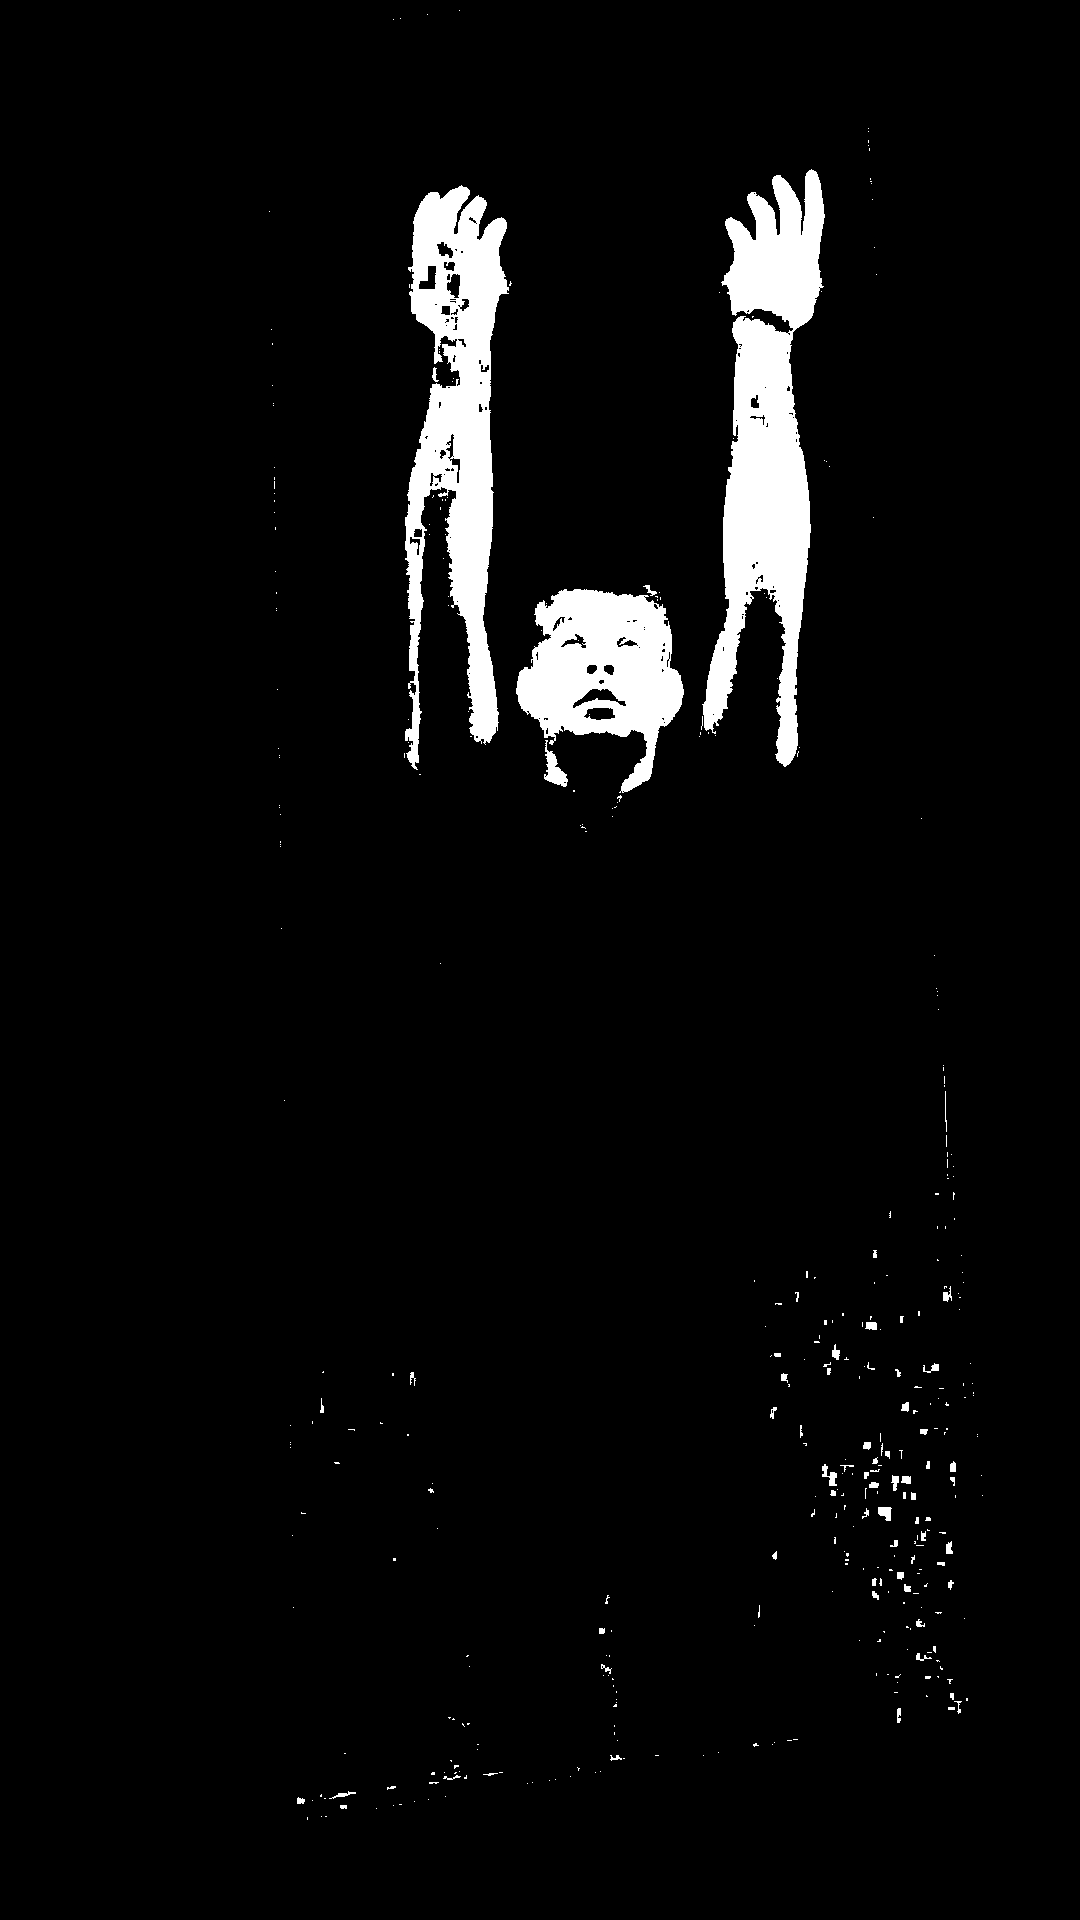
\includegraphics[scale=0.1]{img/desenvolvimento/maoBarra/limited.png}
    \caption*{Fonte - Próprio Autor.}
    \end{figure}
\end{frame}


\begin{frame}{Mão na barra - Desfoque}
    \begin{figure}[!ht]
    \centering
    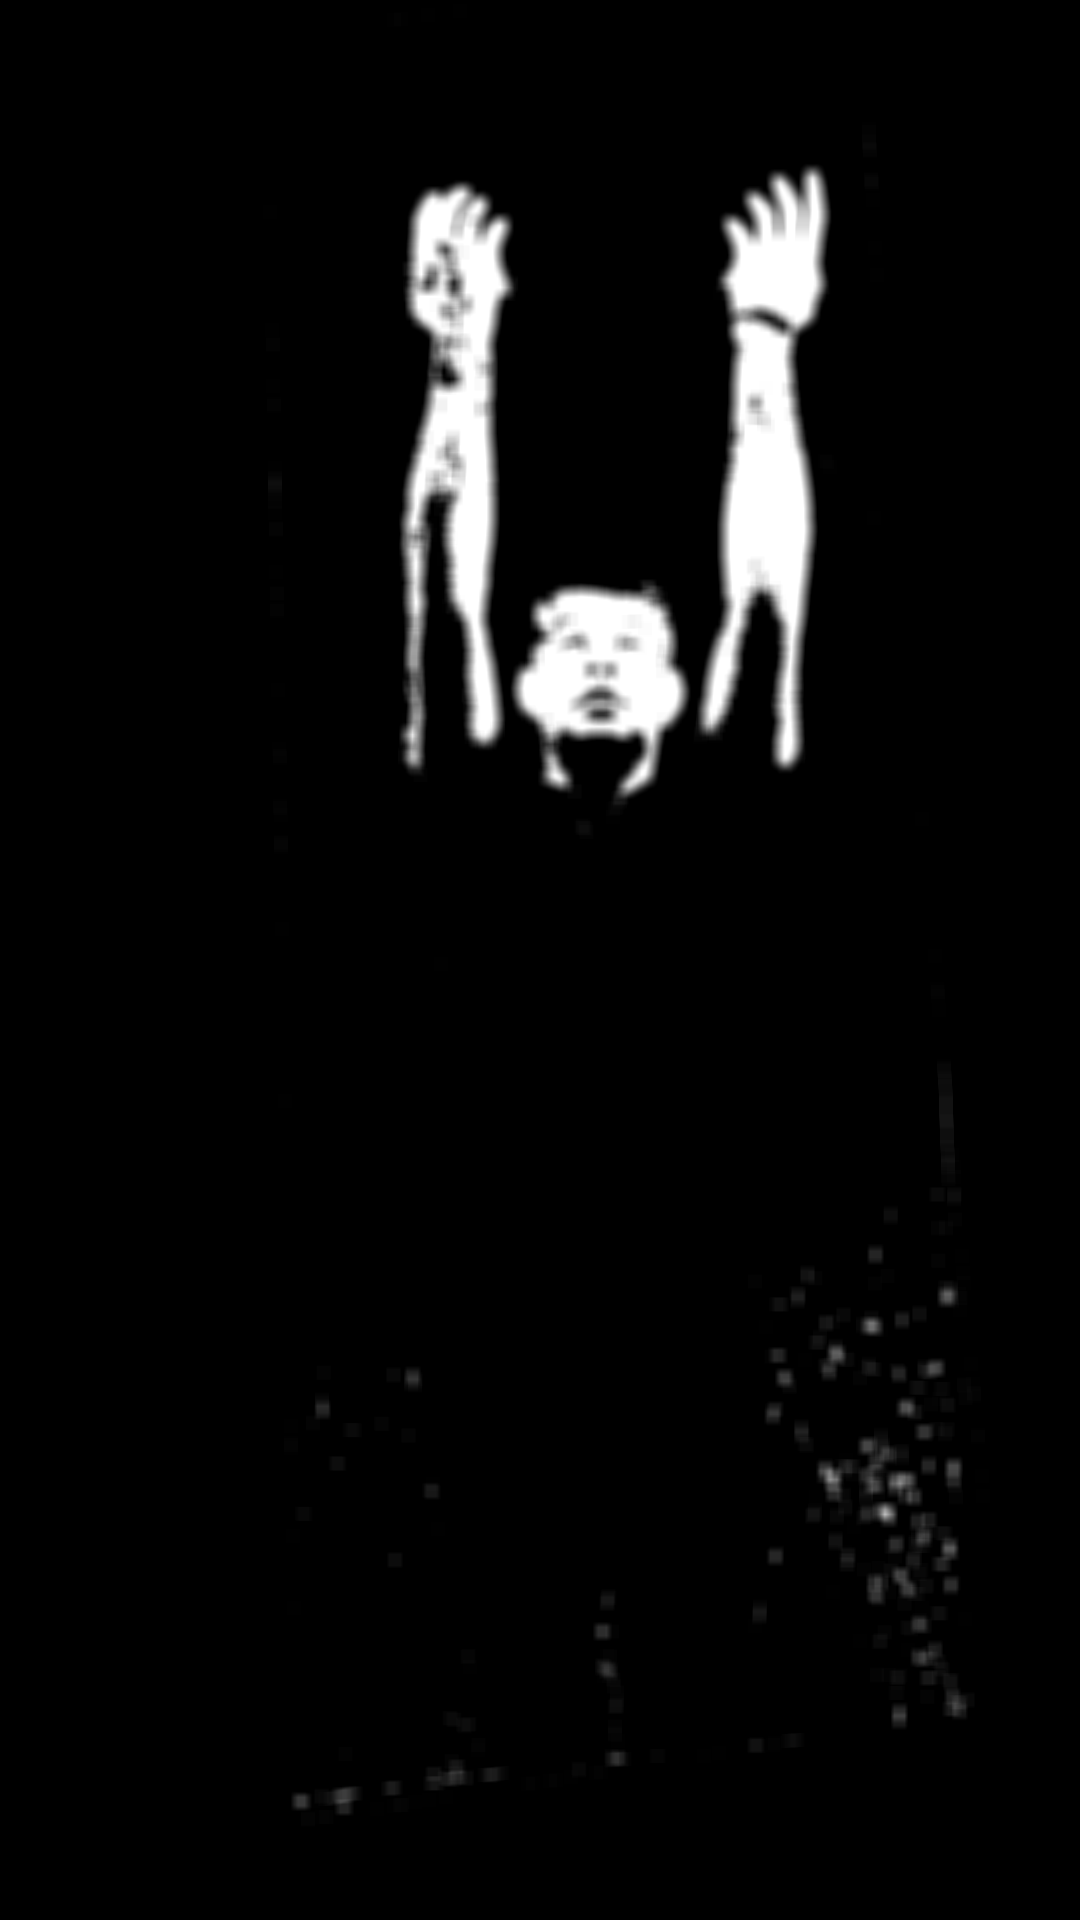
\includegraphics[scale=0.1]{img/desenvolvimento/maoBarra/blur.png}
    \caption*{Fonte - Próprio Autor.}
    \end{figure}
\end{frame}


\begin{frame}{Mão na barra - 2º Limiarização}
    \begin{figure}[!ht]
    \centering
    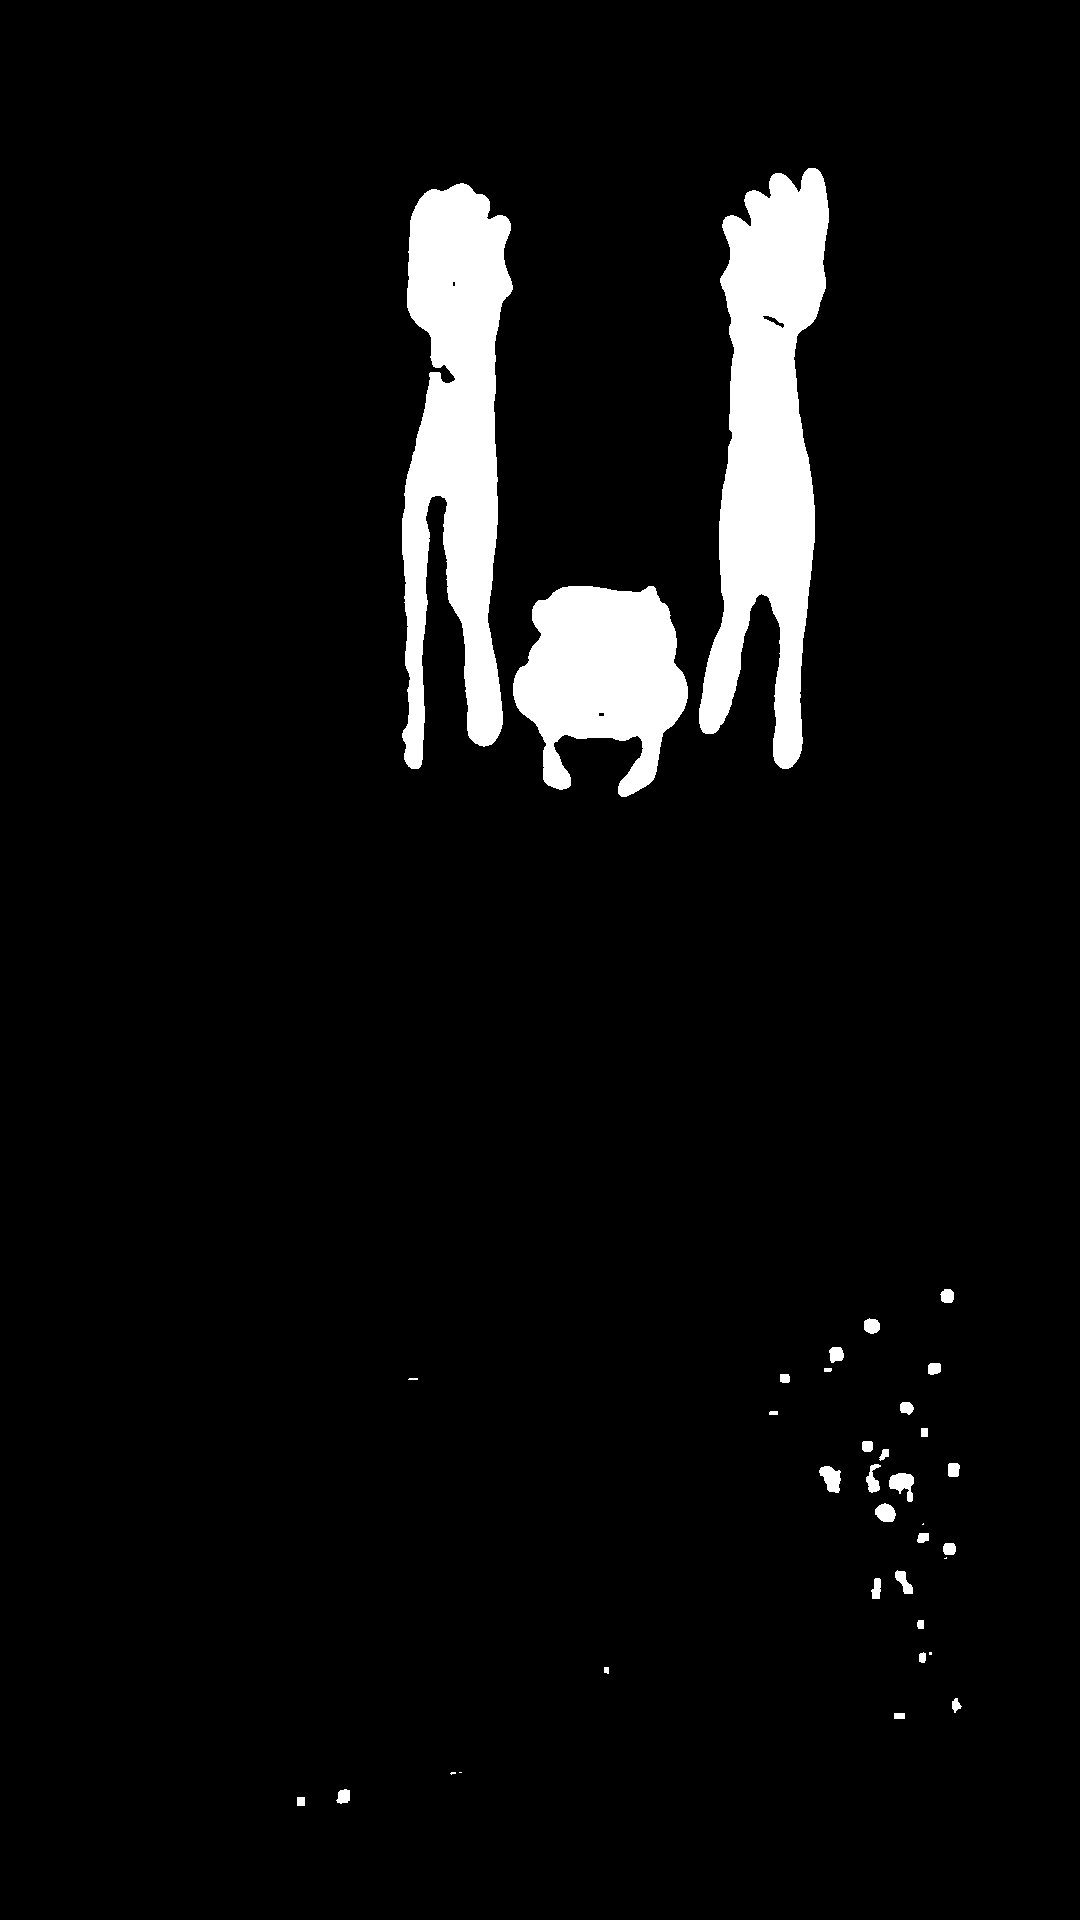
\includegraphics[scale=0.1]{img/desenvolvimento/maoBarra/limited2.png}
    \caption*{Fonte - Próprio Autor.}
    \end{figure}
\end{frame}

\begin{frame}{Mão na barra - Pixel}
    \begin{figure}[!ht]
    \centering
    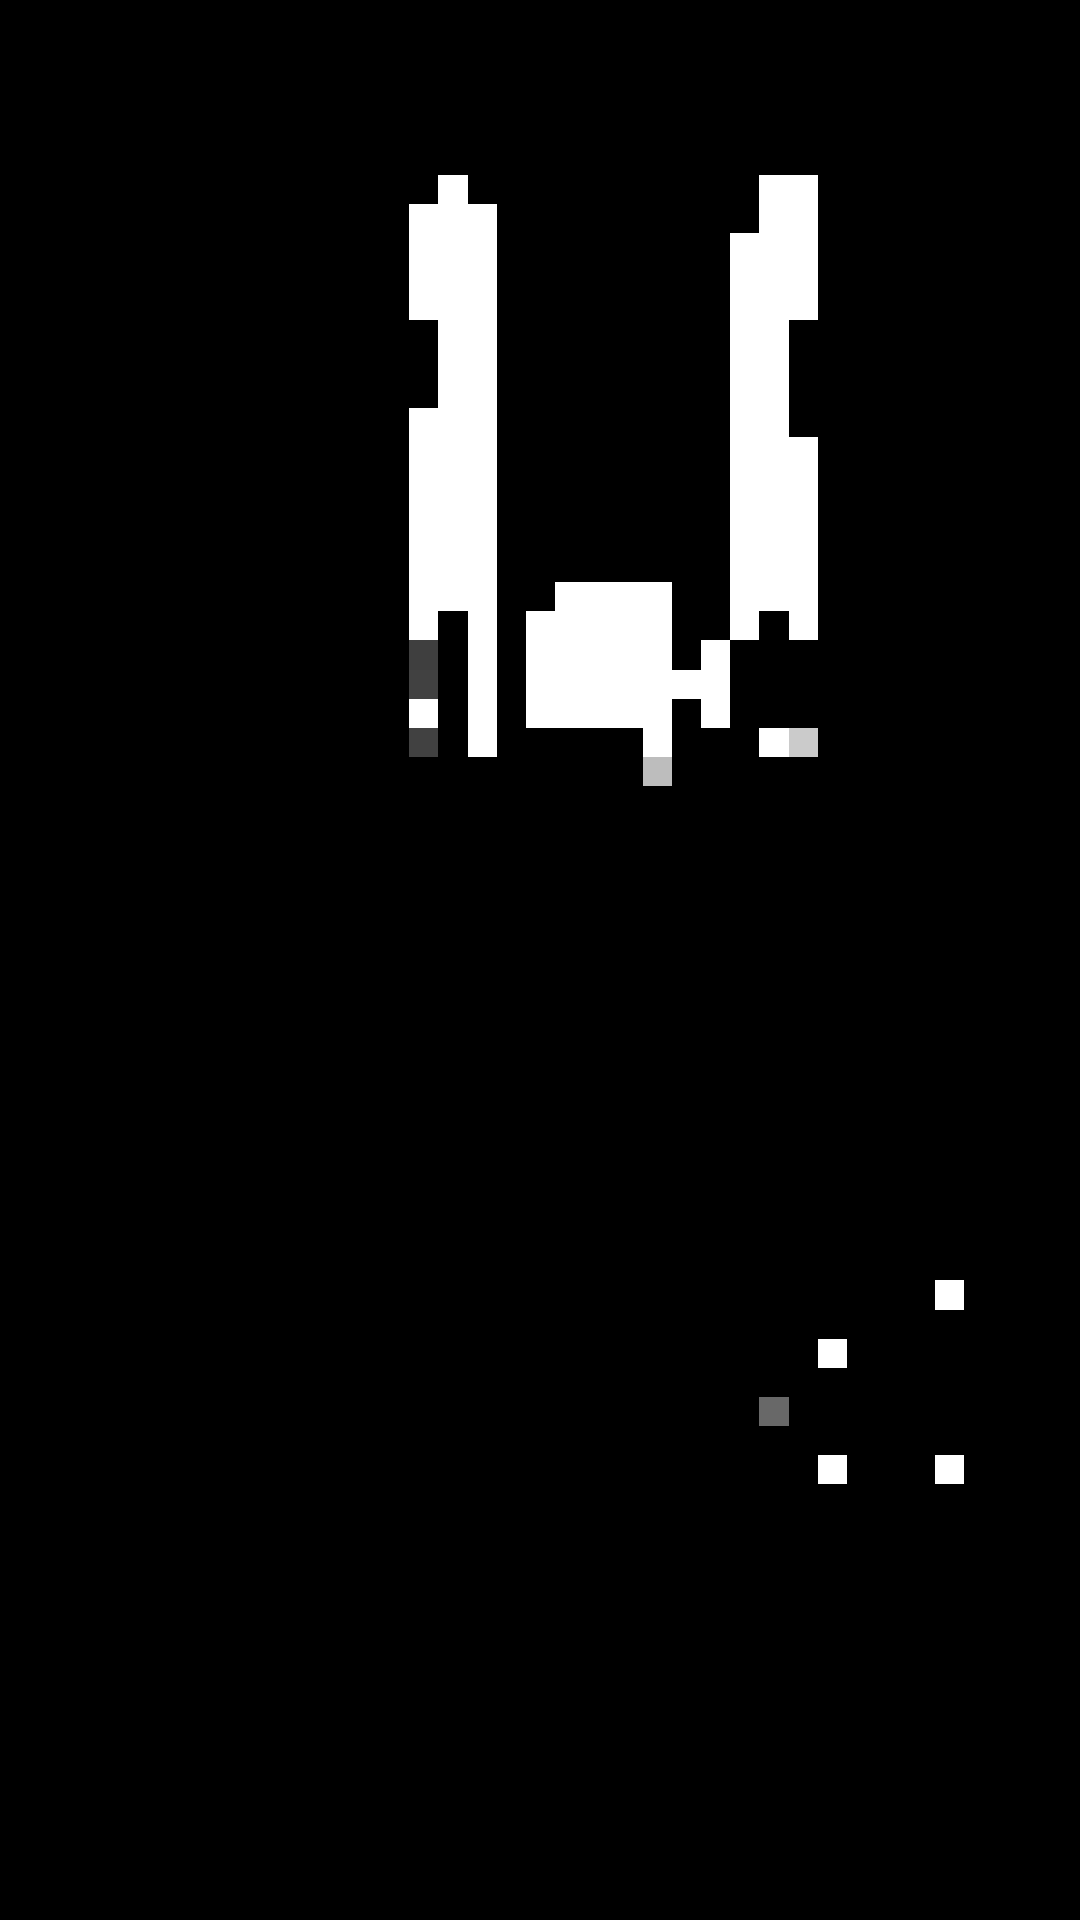
\includegraphics[scale=0.1]{img/desenvolvimento/maoBarra/pixel.png}
    \caption*{Fonte - Próprio Autor.}
    \end{figure}
\end{frame}


\begin{frame}{Mão na barra - 3º Limiarização}
    \begin{figure}[!ht]
    \centering
    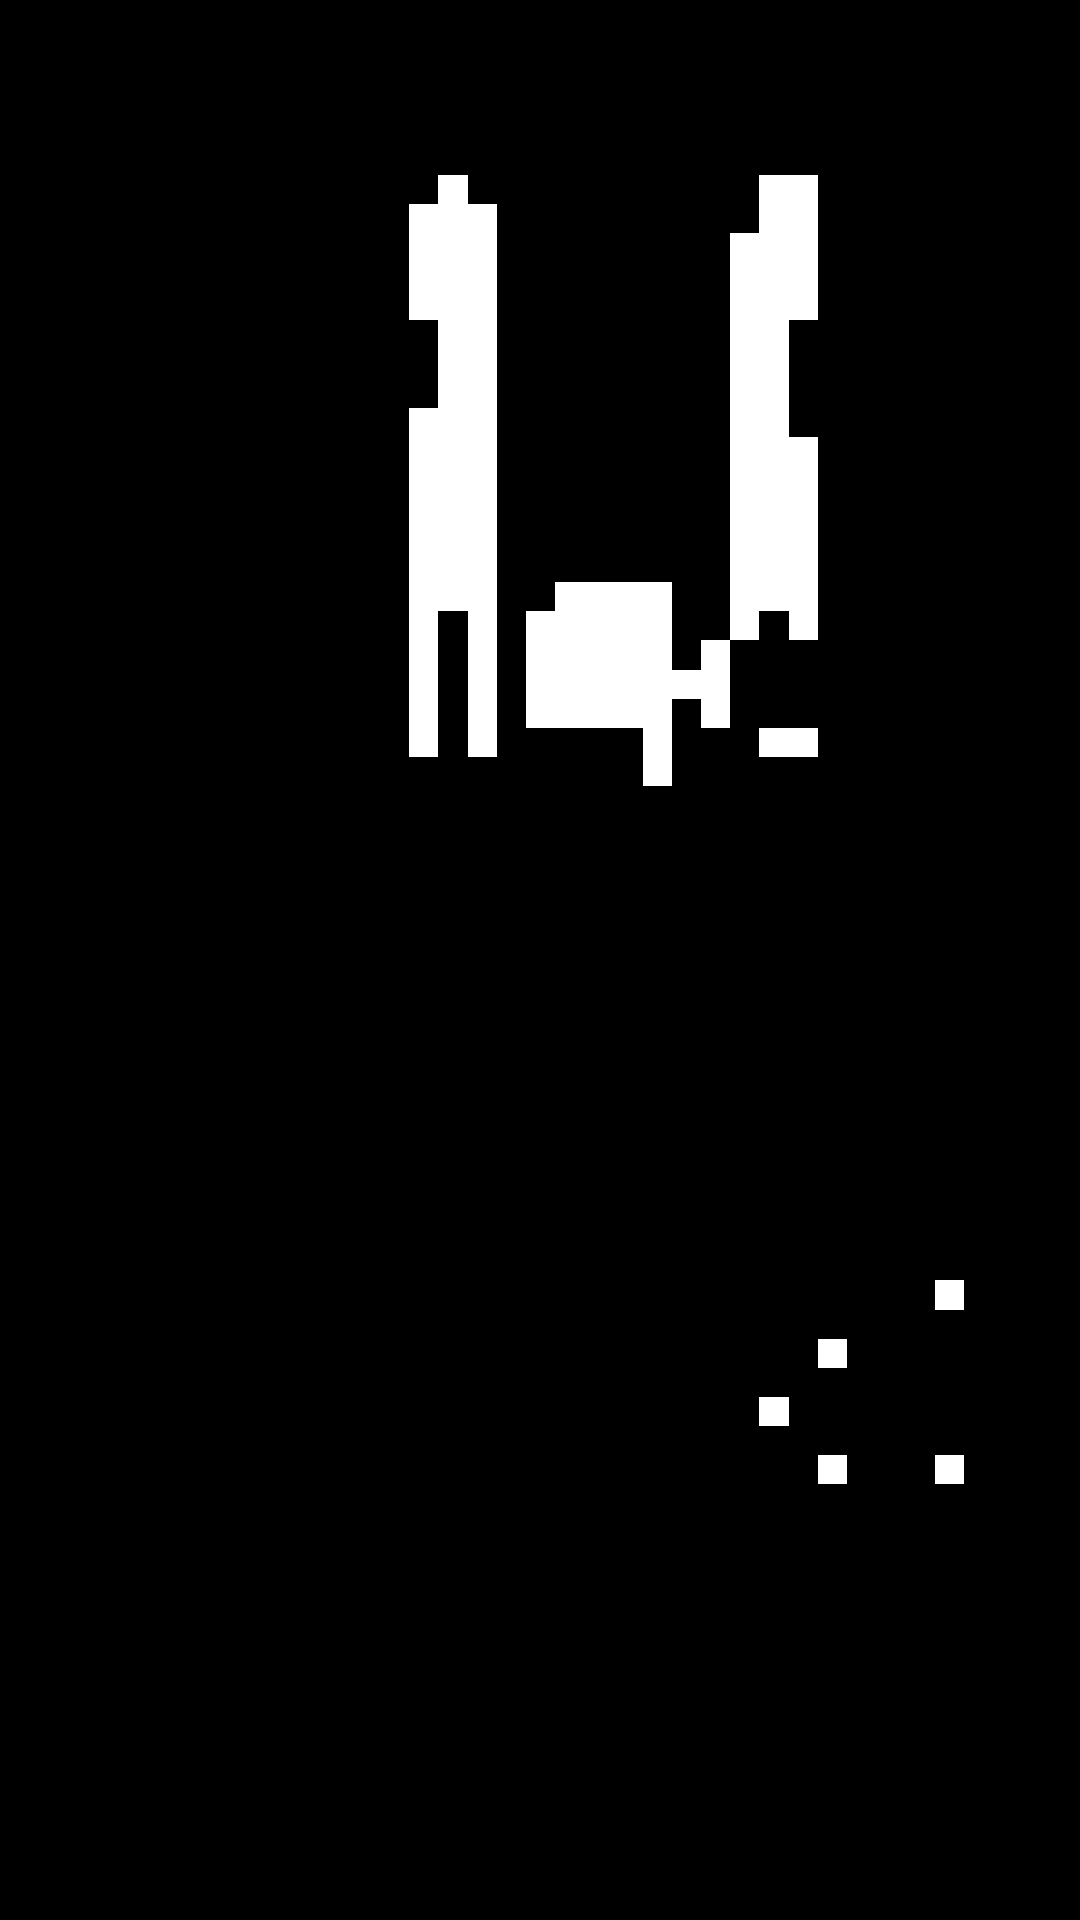
\includegraphics[scale=0.1]{img/desenvolvimento/maoBarra/limited3.png}
    \caption*{Fonte - Próprio Autor.}
    \end{figure}
\end{frame}

\begin{frame}{Mão na barra - Máscara da região de interesse}
    \begin{figure}[!ht]
    \centering
    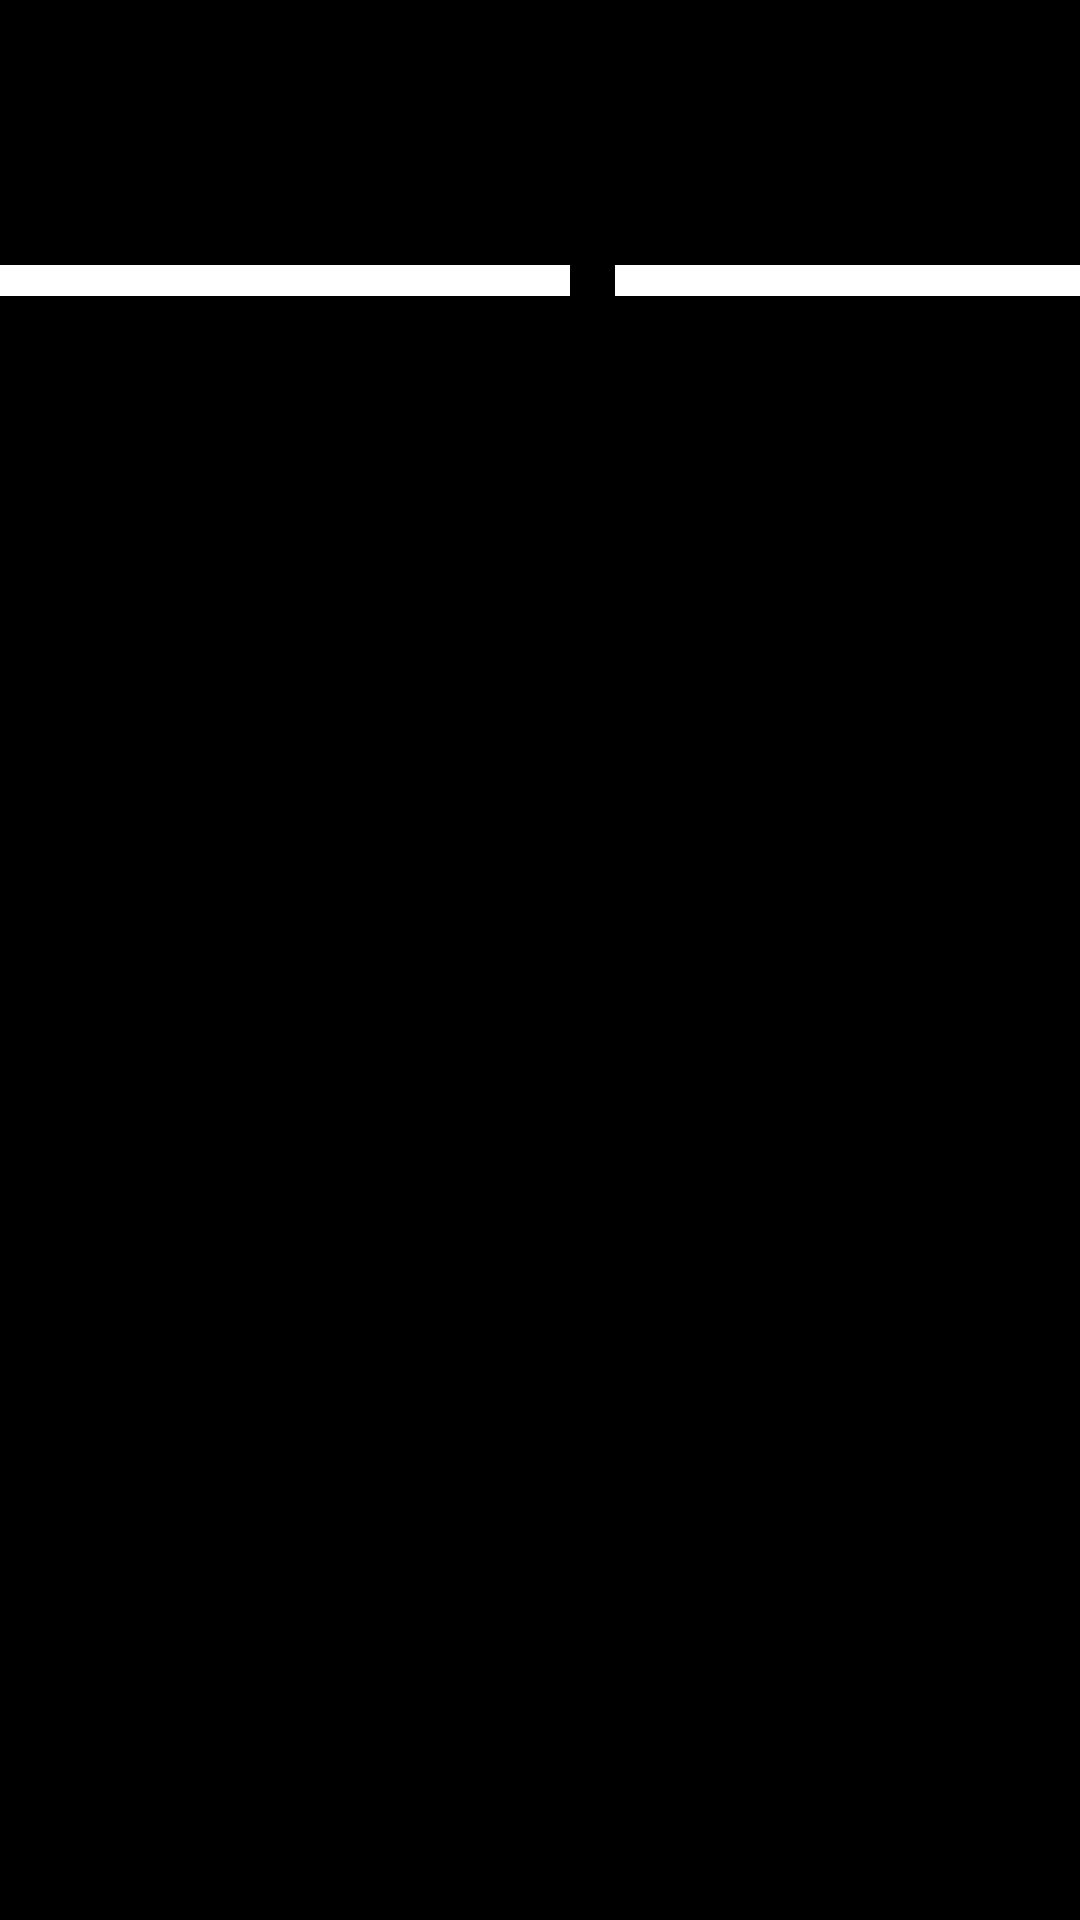
\includegraphics[scale=0.1]{img/desenvolvimento/maoBarra/mask3.png}
    \caption*{Fonte - Próprio Autor.}
    \end{figure}
\end{frame}

\begin{frame}{Mão na barra - Imagem segmentada}
    \begin{figure}[!ht]
    \centering
    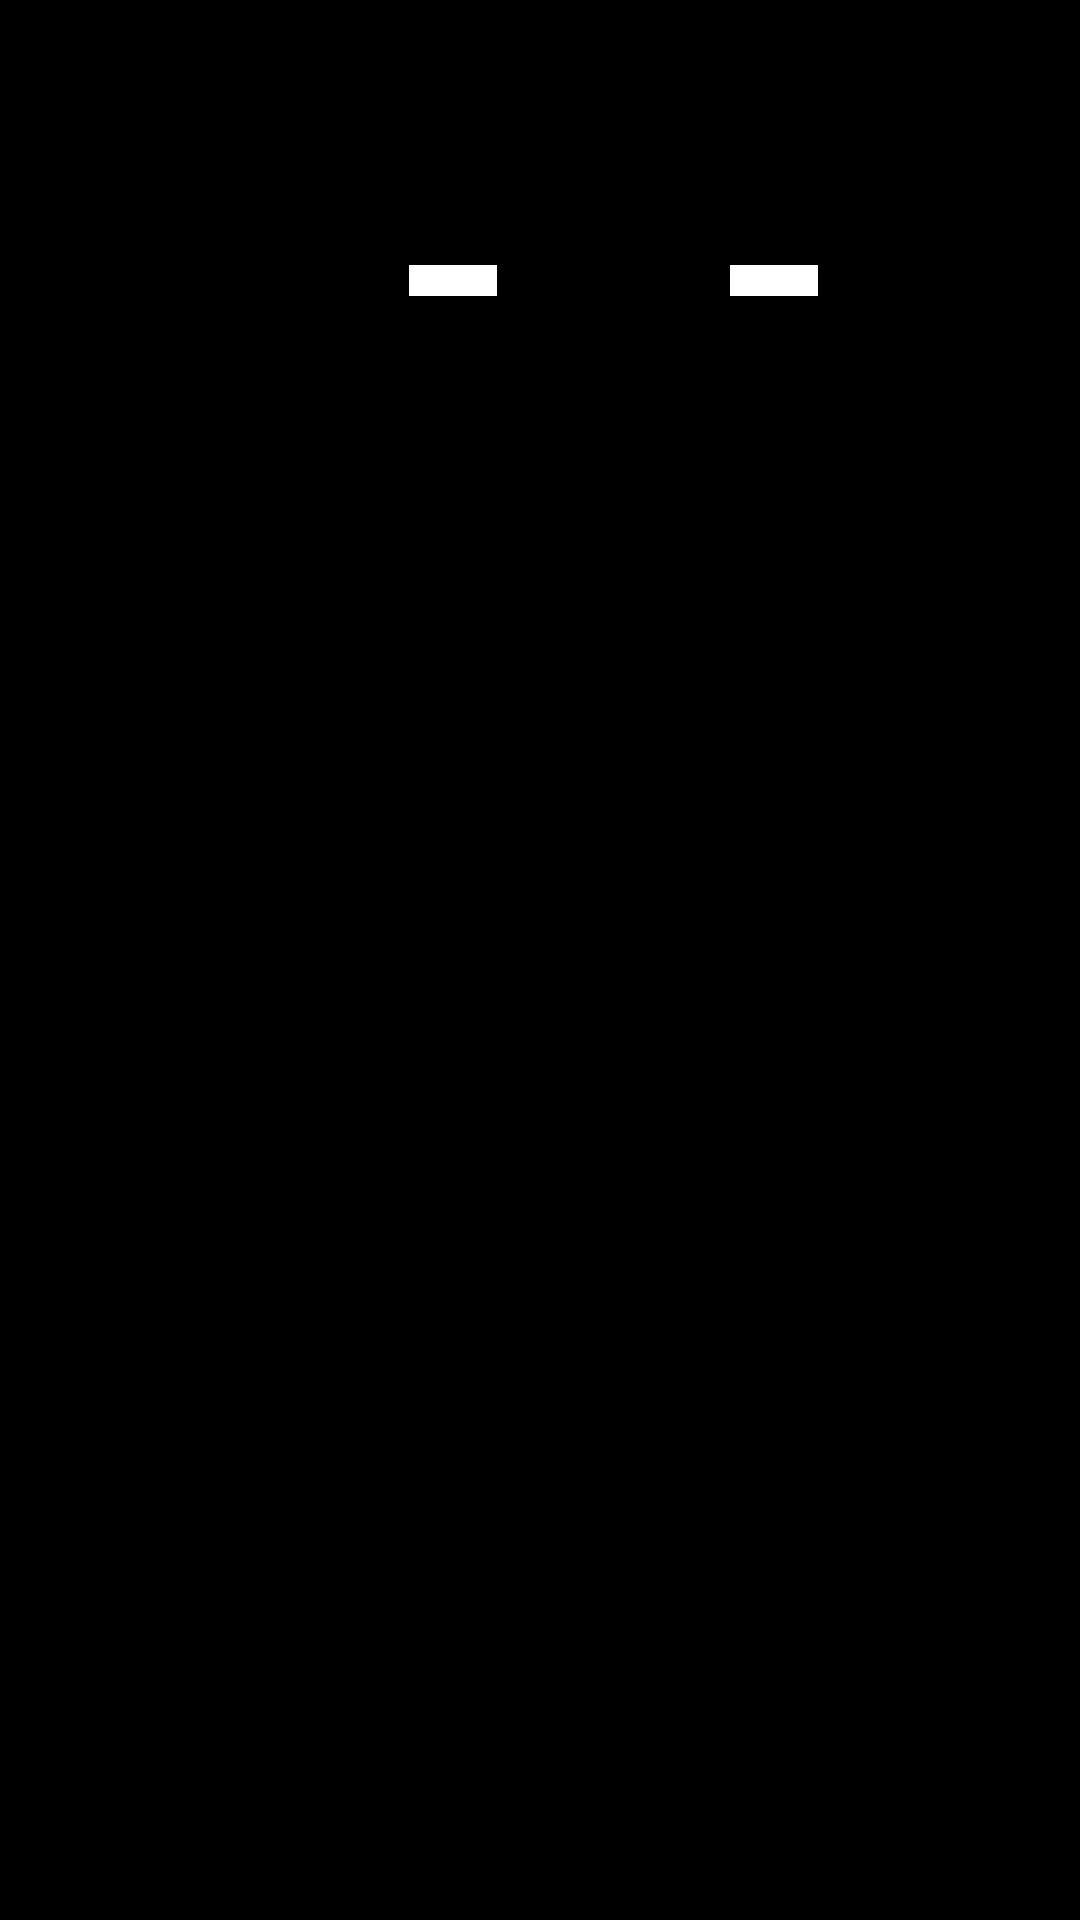
\includegraphics[scale=0.1]{img/desenvolvimento/maoBarra/only_hands.png}
    \caption*{Fonte - Próprio Autor.}
    \end{figure}
\end{frame}


\begin{frame}{Mão na barra - Representação}
    \begin{figure}[!ht]
    \centering
    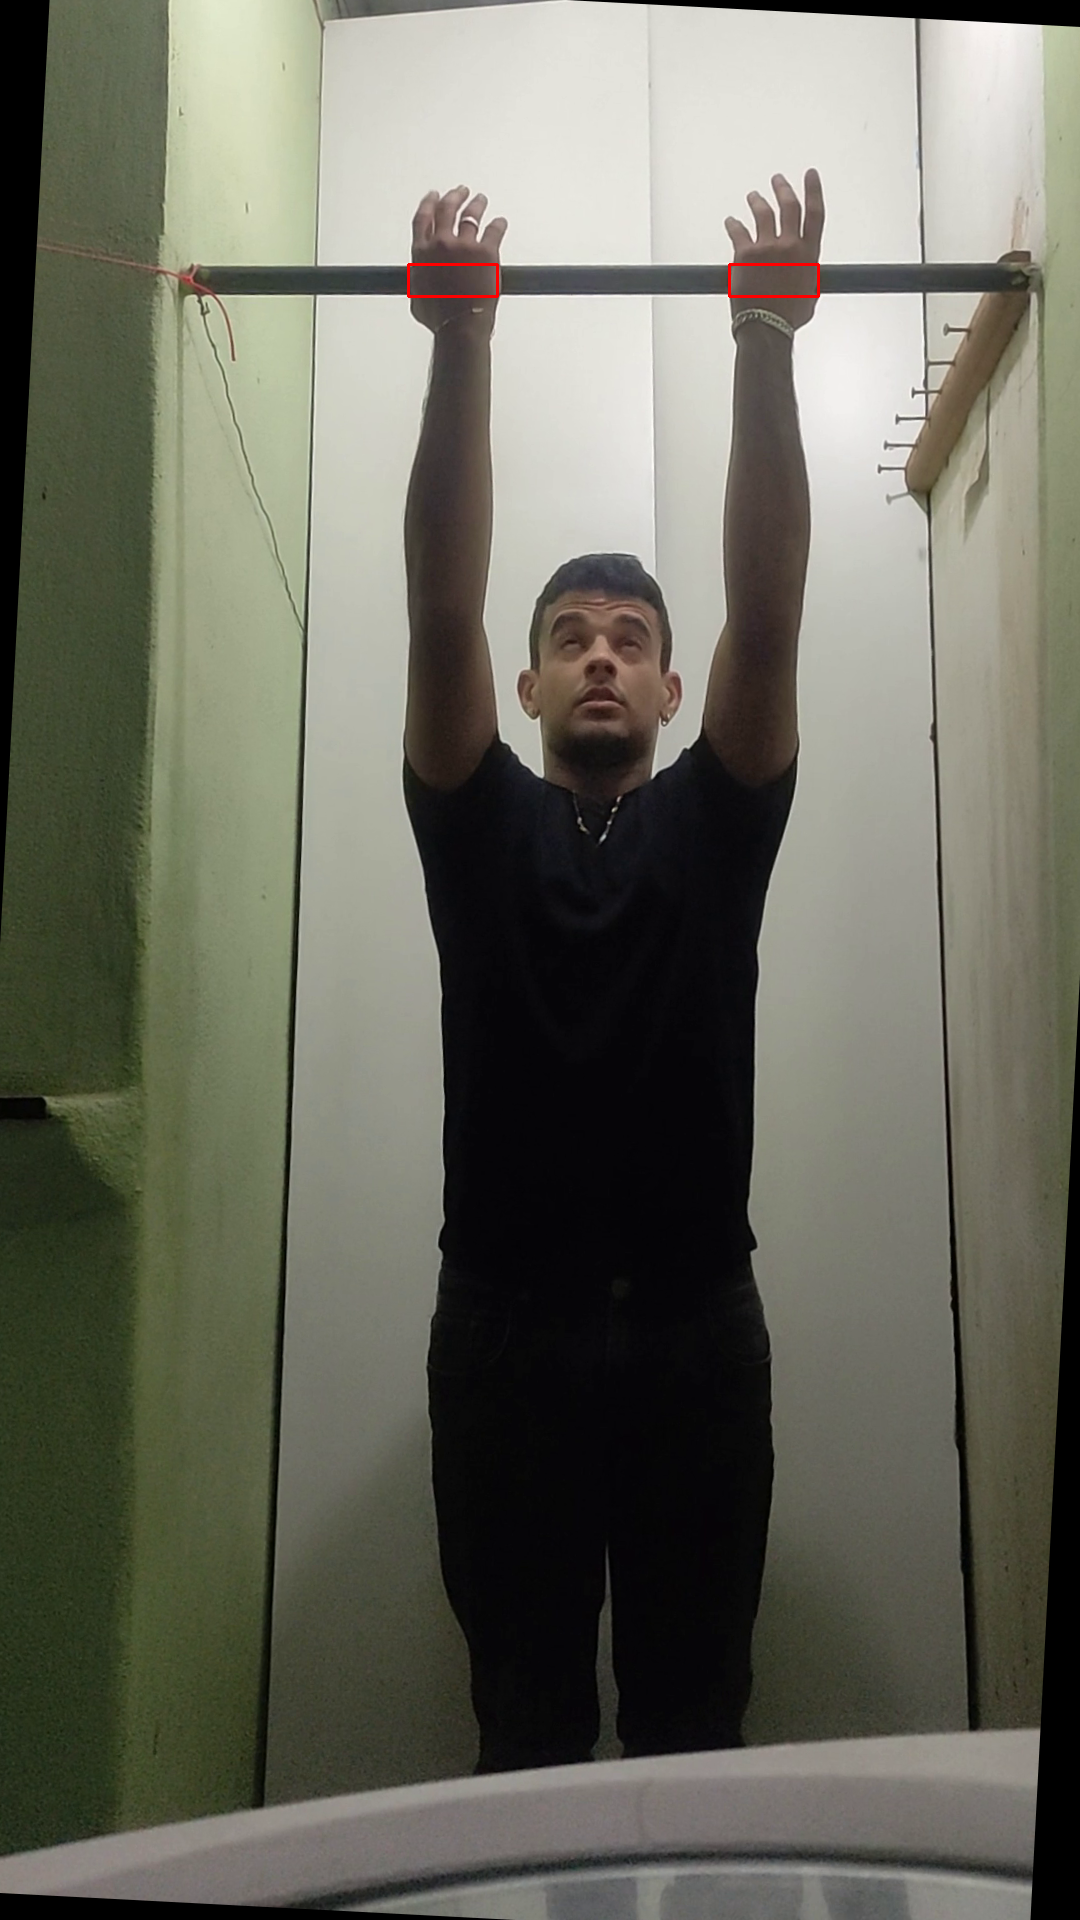
\includegraphics[scale=0.1]{img/desenvolvimento/maoBarra/contornos.png}
    \caption*{Fonte - Próprio Autor.}
    \end{figure}
\end{frame}



%%%%%%%%%%%%%%%%%%%%%%%%%%%%%%%%%%%%%%%%%%%%%%%%%%%%%%%%%%%%%%%%%%%%
%%
%%                     Braço esticado
%%
%%%%%%%%%%%%%%%%%%%%%%%%%%%%%%%%%%%%%%%%%%%%%%%%%%%%%%%%%%%%%%%%%%%%


\begin{frame}{Braço esticado - Fluxograma}
    \begin{figure}[!ht]
        \centering
            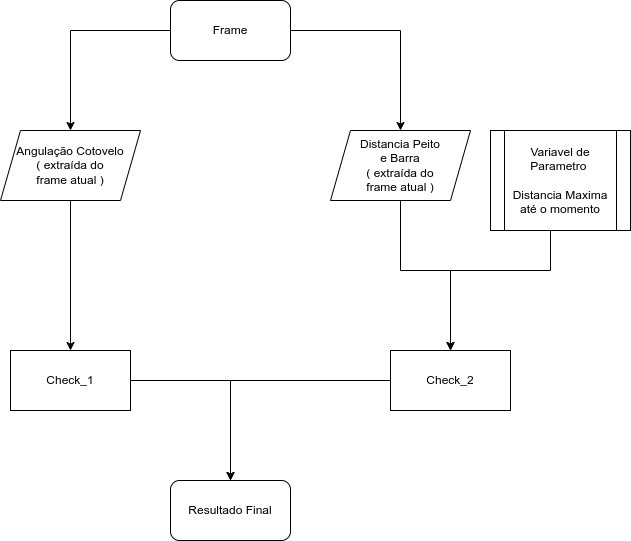
\includegraphics[scale=0.35]{img/desenvolvimento/bracoEsticado/fluxograma.png}
        \caption*{Fonte - Próprio Autor.}
    \end{figure}
\end{frame}


\begin{frame}{Braço esticado - Segmento dos membros}
    \begin{figure}[!ht]
        \centering
            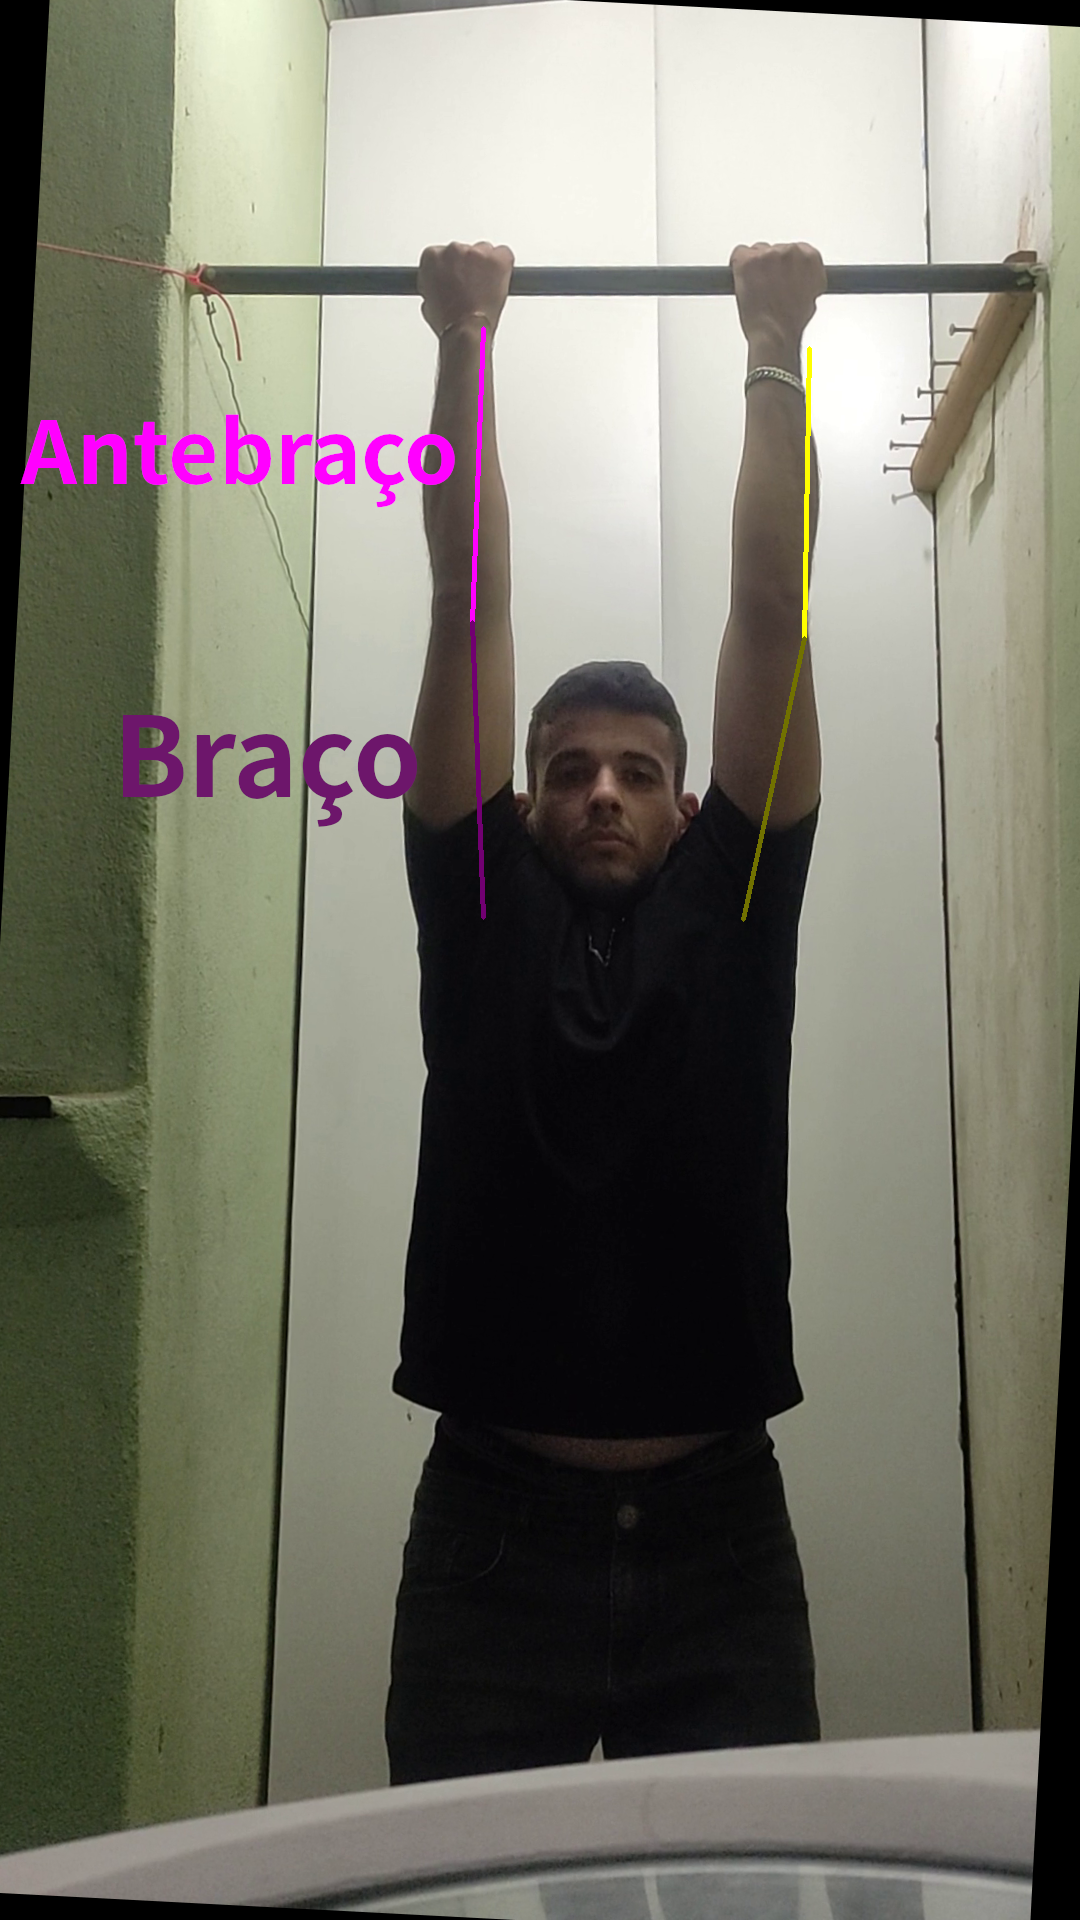
\includegraphics[scale=0.1]{img/desenvolvimento/bracoEsticado/bracoEsticado.png}
        \caption*{Fonte - Próprio Autor.}
    \end{figure}
\end{frame}

\begin{frame}{Braço esticado - Imprecisão}
    \begin{itemize}
        \item É aceito até 13 graus de movimento.
    \end{itemize}
\end{frame}

\begin{frame}{Braço esticado - Ombros}
    \begin{figure}[!ht]
        \centering
            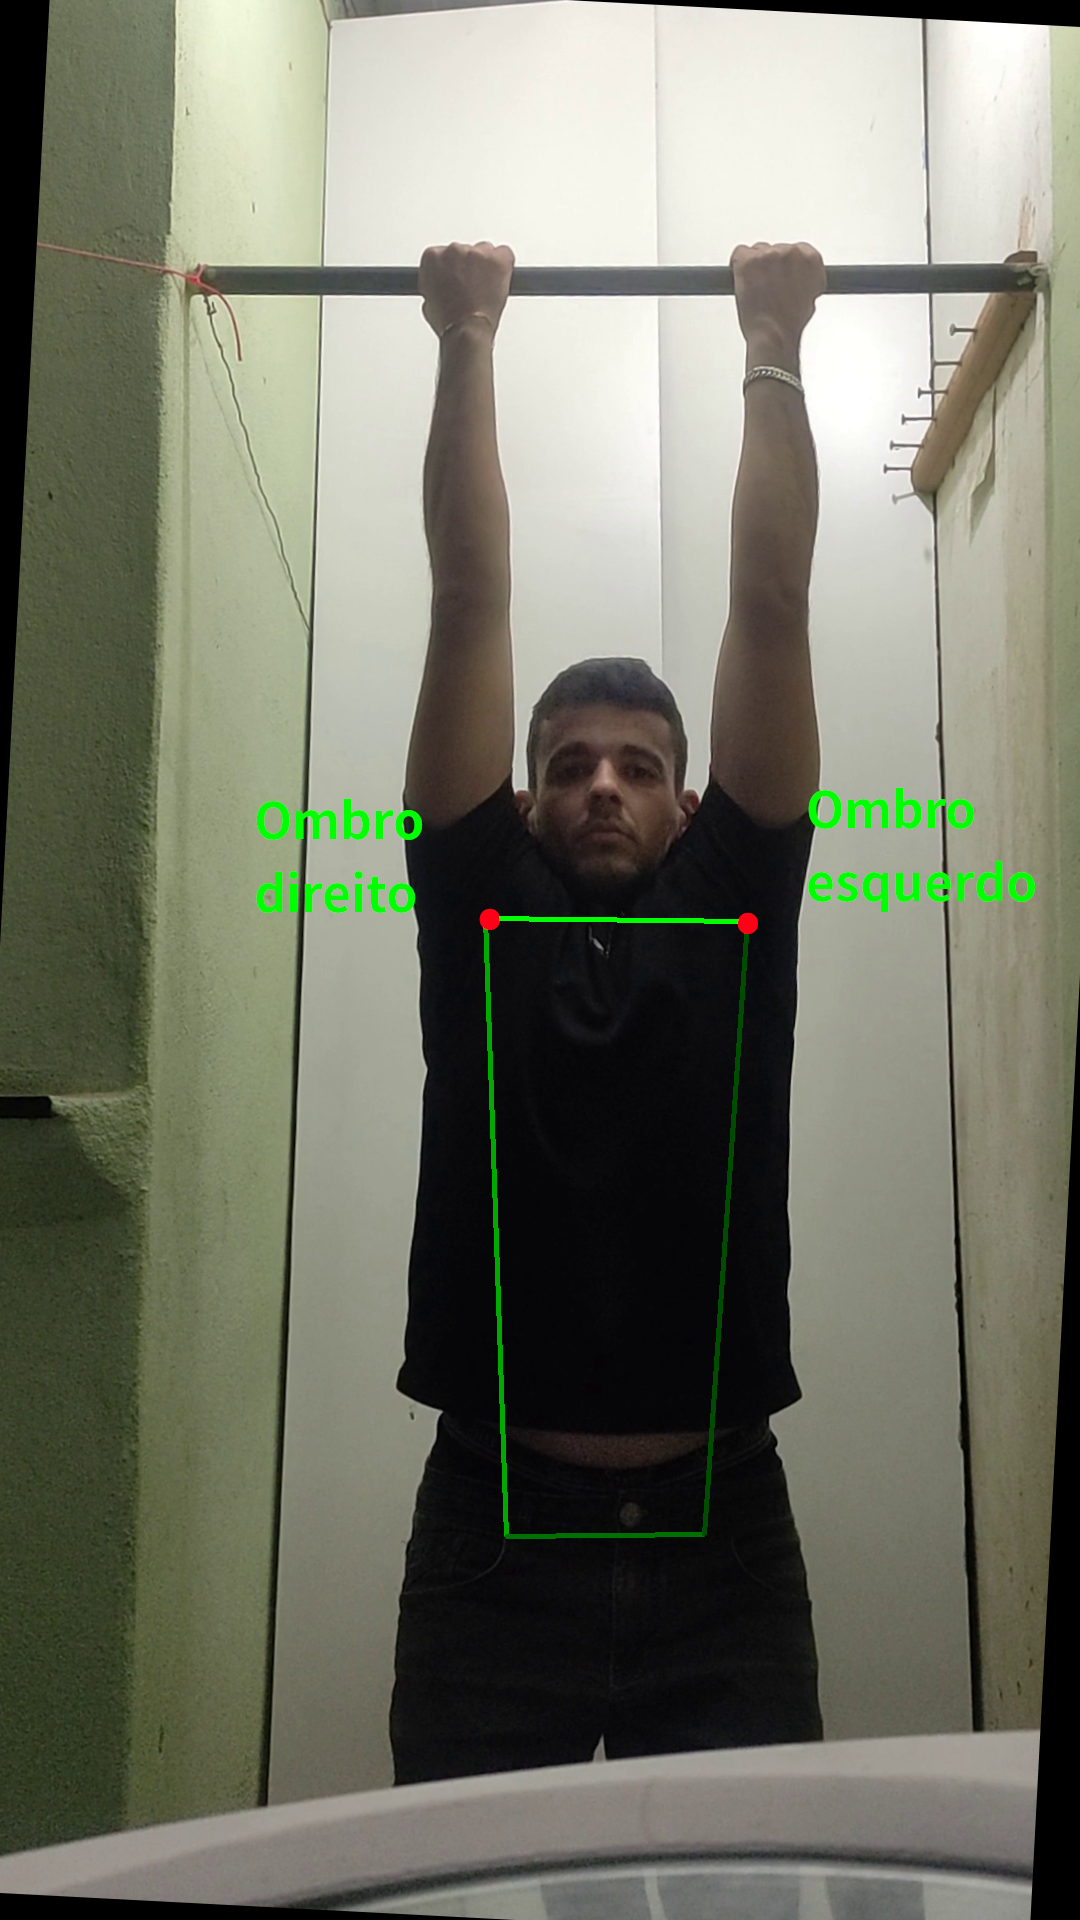
\includegraphics[scale=0.1]{img/desenvolvimento/bracoEsticado/tronco.png}
        \caption*{Fonte - Próprio Autor.}
    \end{figure}
\end{frame}



%%%%%%%%%%%%%%%%%%%%%%%%%%%%%%%%%%%%%%%%%%%%%%%%%%%%%%%%%%%%%%%%%%%%
%%
%%                     Ultrapassagem do queixo a barra
%%
%%%%%%%%%%%%%%%%%%%%%%%%%%%%%%%%%%%%%%%%%%%%%%%%%%%%%%%%%%%%%%%%%%%%

\begin{frame}{Ultrapassagem do queixo à barra - Fluxograma}
    \begin{figure}[!ht]
        \centering
            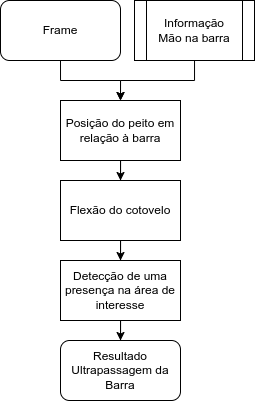
\includegraphics[scale=0.42]{img/desenvolvimento/ultrapassagemBarra/fluxograma.png}
        \caption*{Fonte - Próprio Autor.}
    \end{figure}
\end{frame}

\begin{frame}{Ultrapassagem do queixo à barra}
    \begin{itemize}
        \item A distância do ombro à barra tem que ser menor ou igual a 1.5 vezes a largura da barra.
        \item O angulo do braço e antebraço pode ter até 5º graus de movimento
    \end{itemize}
\end{frame}


\begin{frame}{Ultrapassagem do queixo à barra - Frame}
    \begin{figure}[!ht]
        \centering
            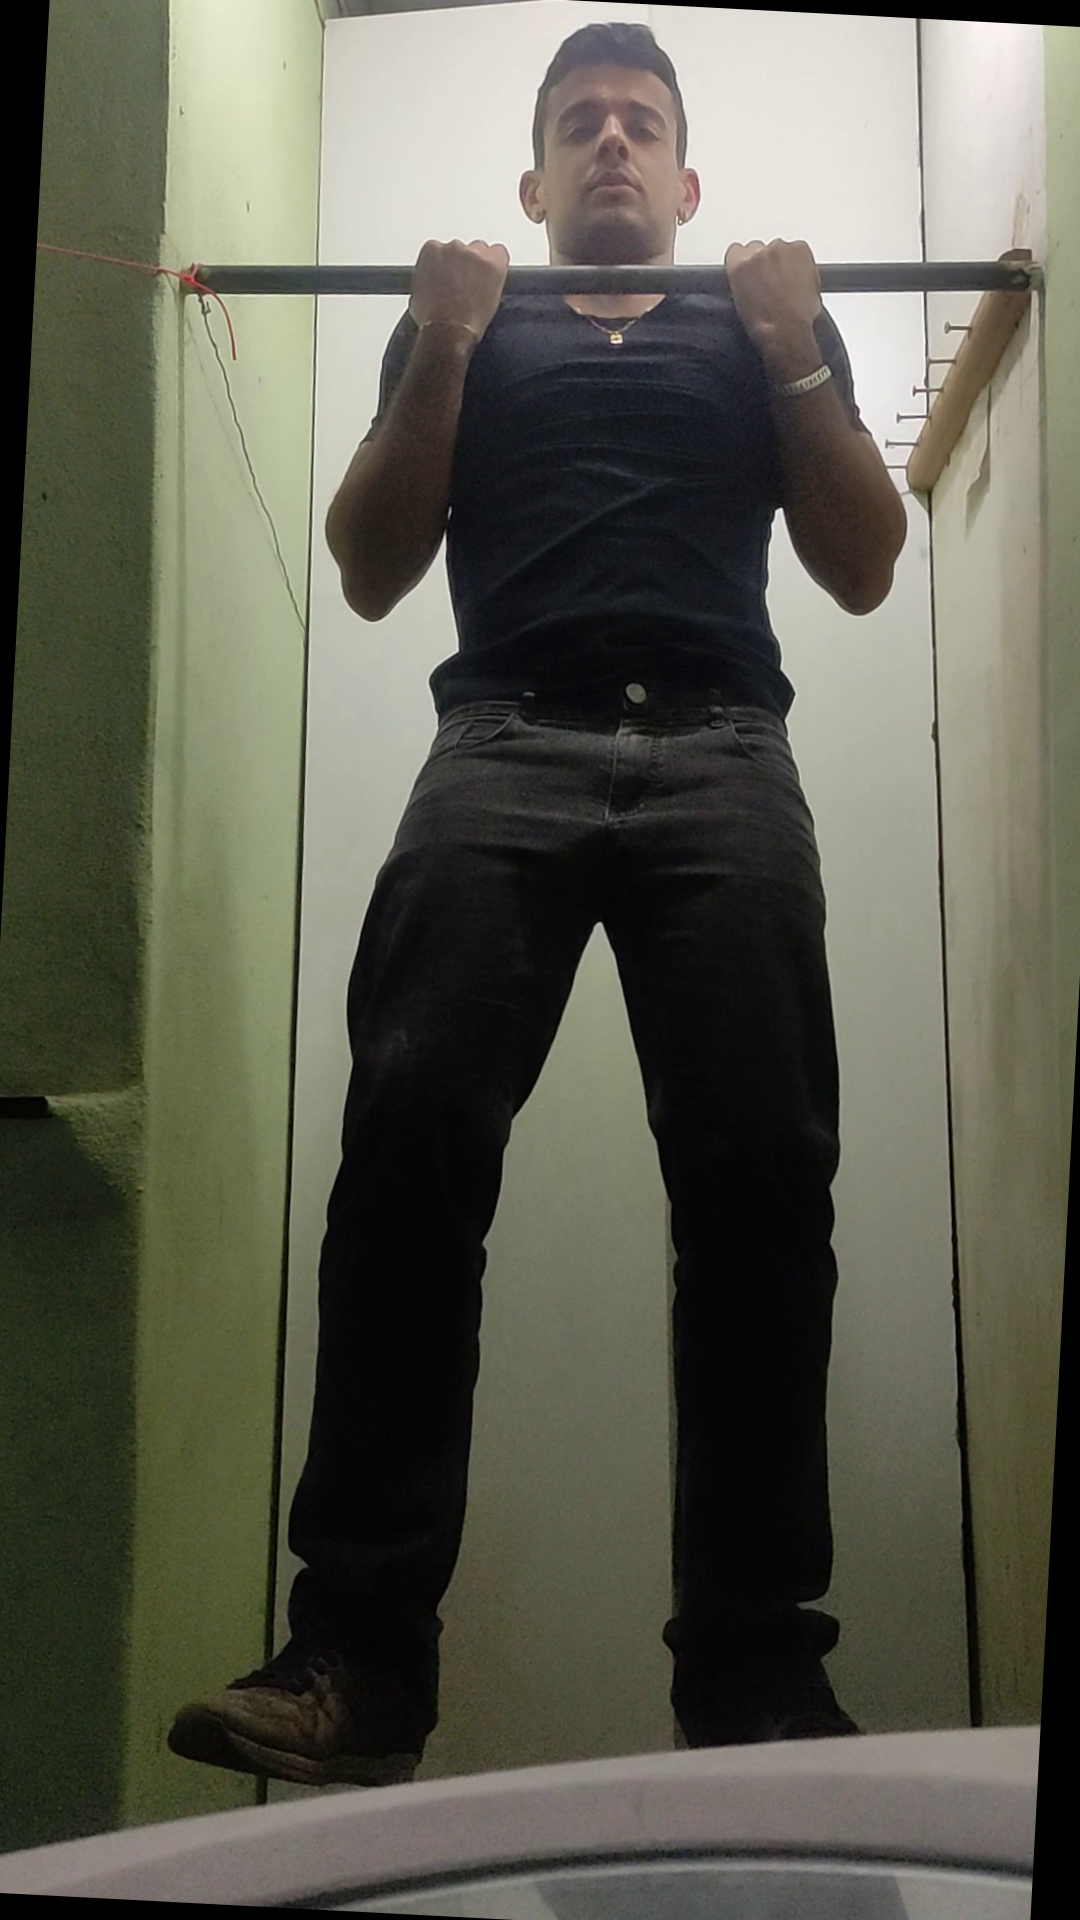
\includegraphics[scale=0.1]{img/desenvolvimento/ultrapassagemBarra/original.png}
        \caption*{Fonte - Próprio Autor.}
    \end{figure}
\end{frame}


\begin{frame}{Ultrapassagem do queixo à barra - Máscara cor da pele}
    \begin{figure}[!ht]
        \centering
            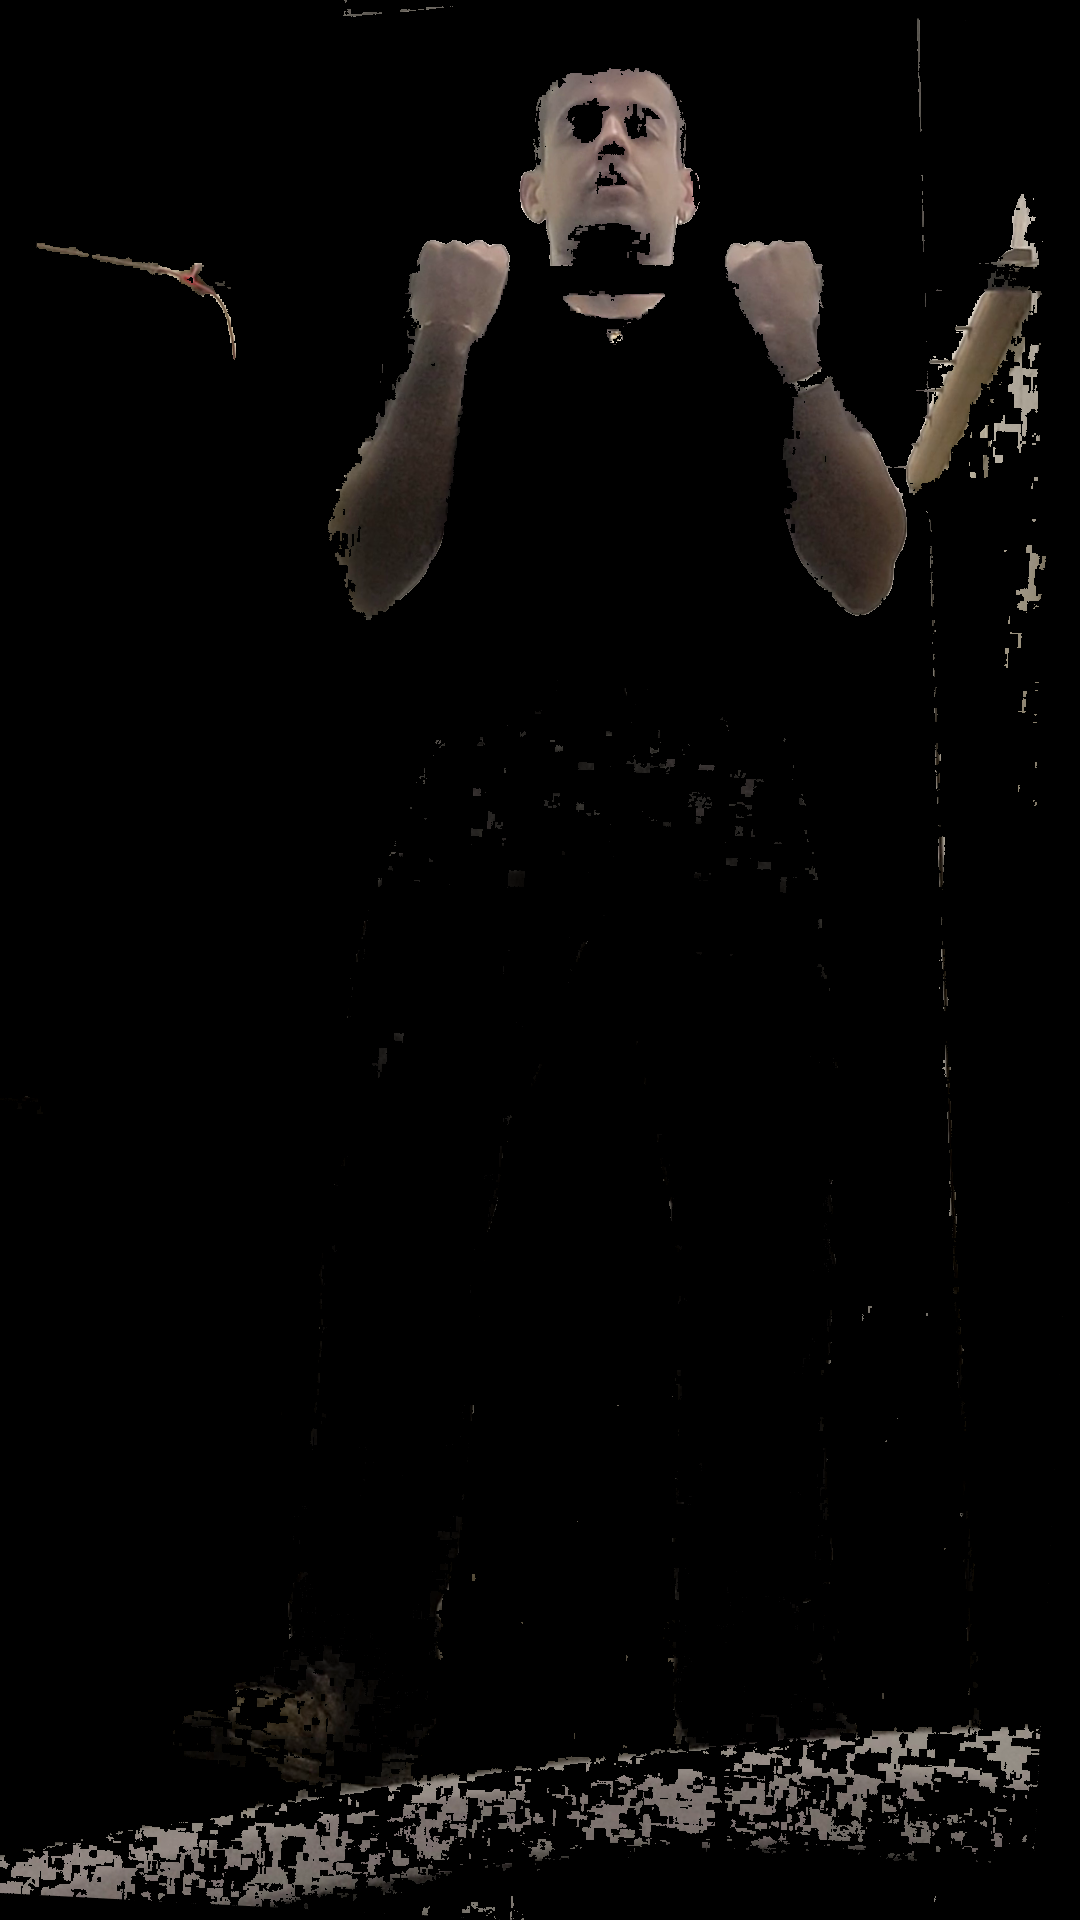
\includegraphics[scale=0.1]{img/desenvolvimento/ultrapassagemBarra/skin.png}
        \caption*{Fonte - Próprio Autor.}
    \end{figure}
\end{frame}

\begin{frame}{Ultrapassagem do queixo à barra - Escala de cinza}
    \begin{figure}[!ht]
        \centering
            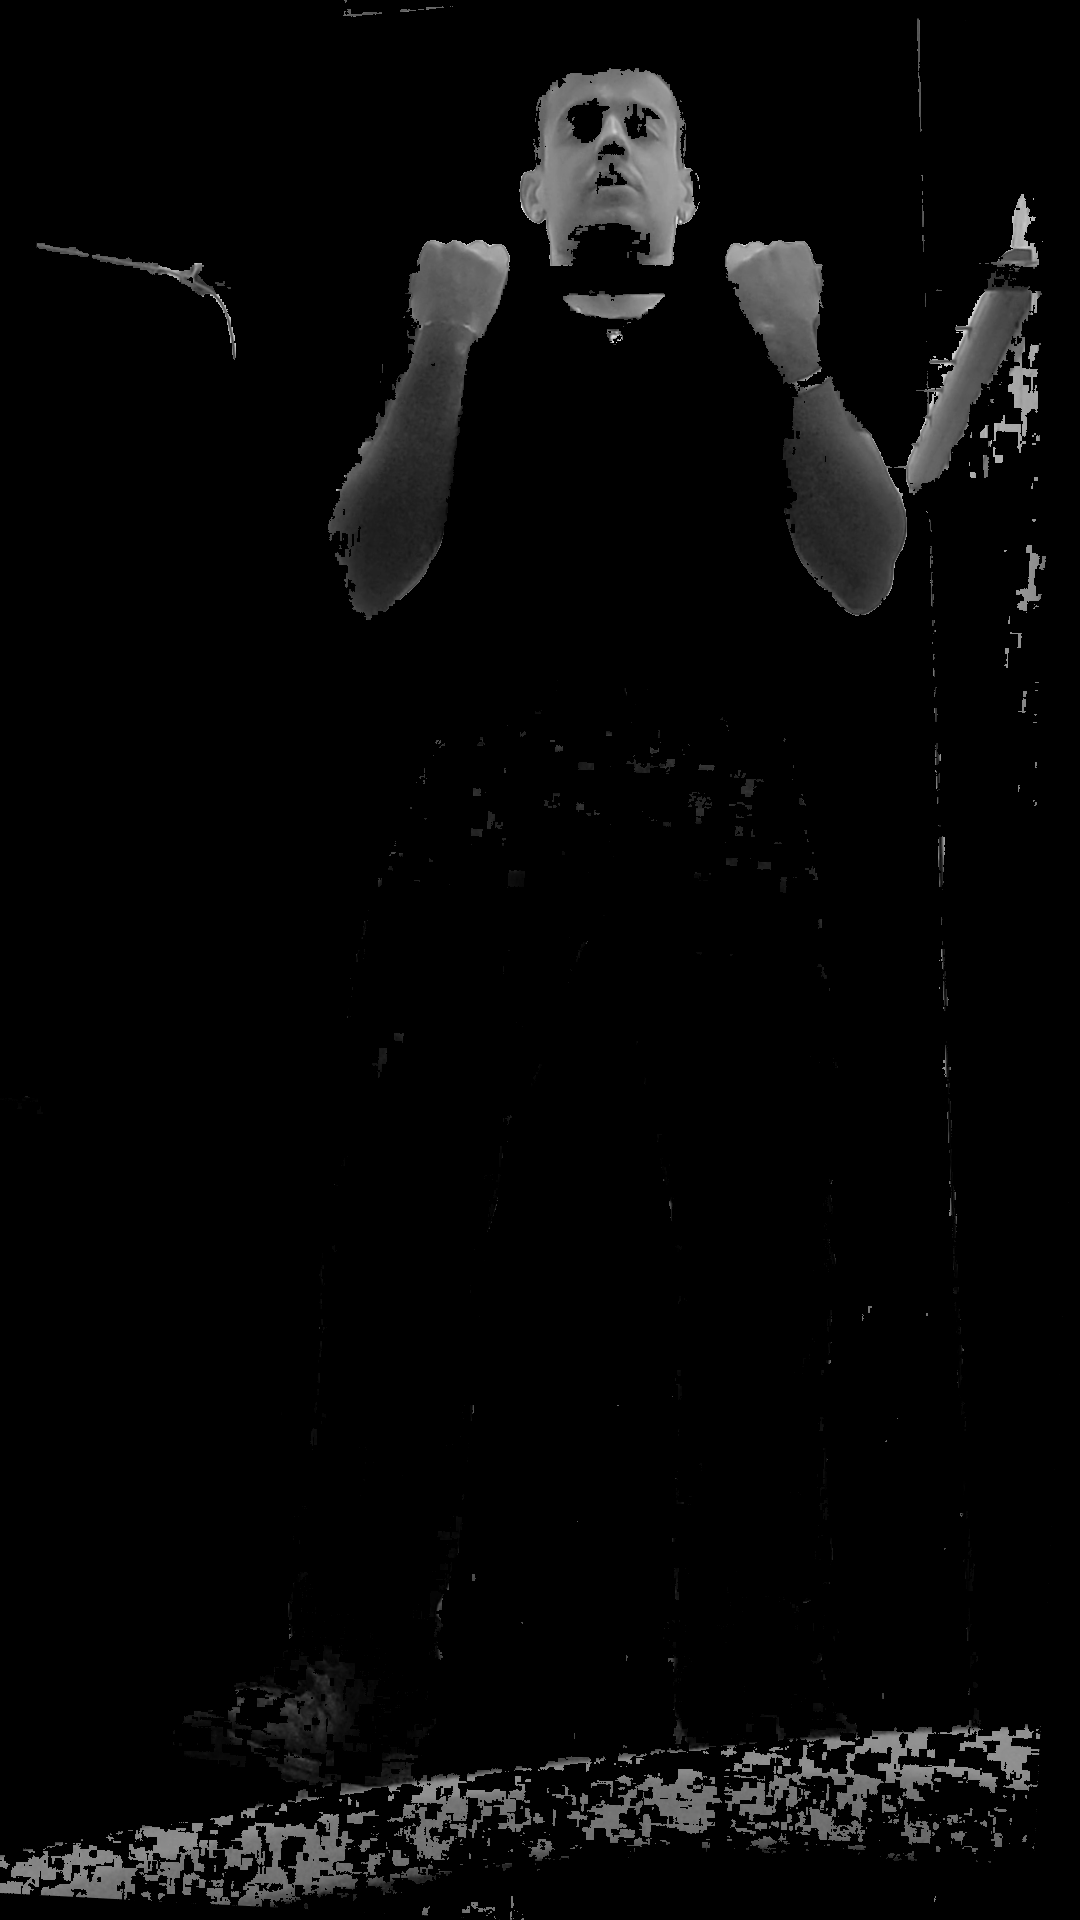
\includegraphics[scale=0.1]{img/desenvolvimento/ultrapassagemBarra/gray.png}
        \caption*{Fonte - Próprio Autor.}
    \end{figure}
\end{frame}

\begin{frame}{Ultrapassagem do queixo à barra - Limiarização}
    \begin{figure}[!ht]
        \centering
            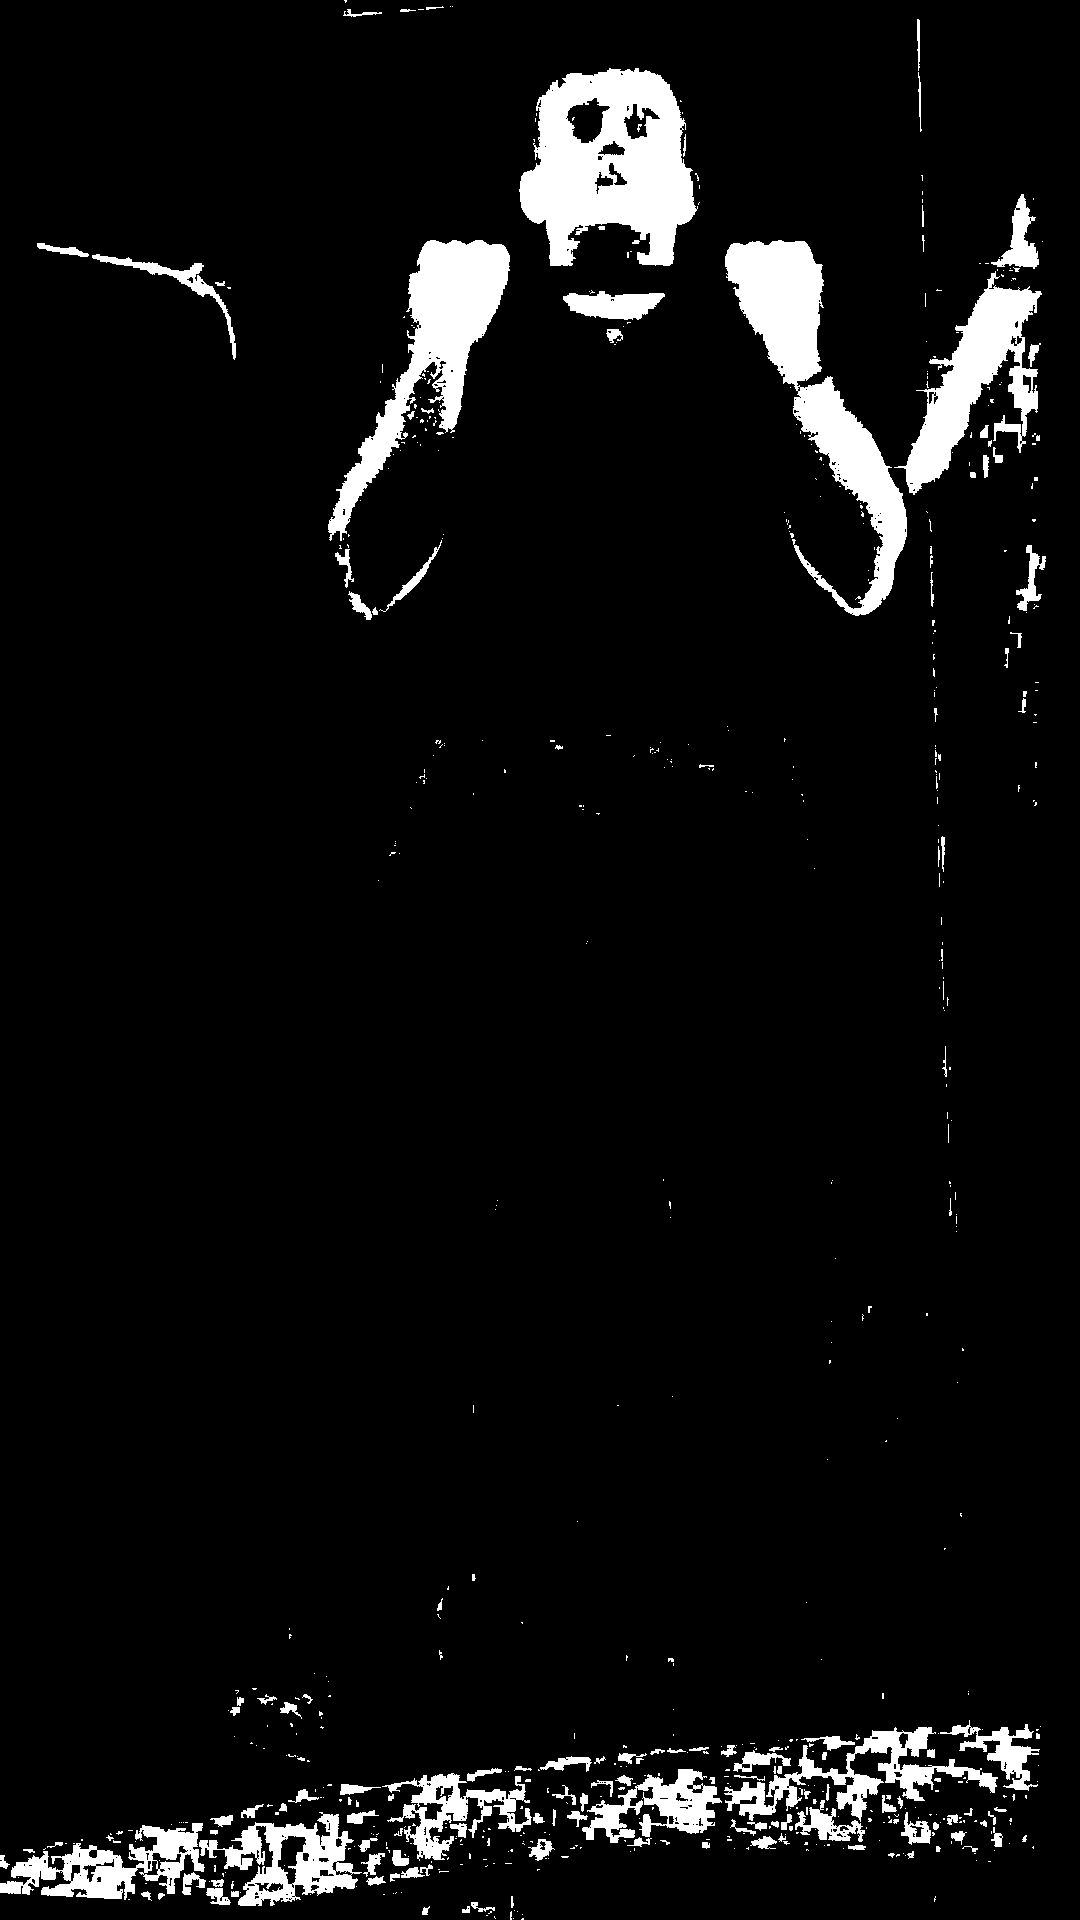
\includegraphics[scale=0.1]{img/desenvolvimento/ultrapassagemBarra/limited.png}
        \caption*{Fonte - Próprio Autor.}
    \end{figure}
\end{frame}


\begin{frame}{Ultrapassagem do queixo à barra - Máscara}
    \begin{figure}[!ht]
        \centering
            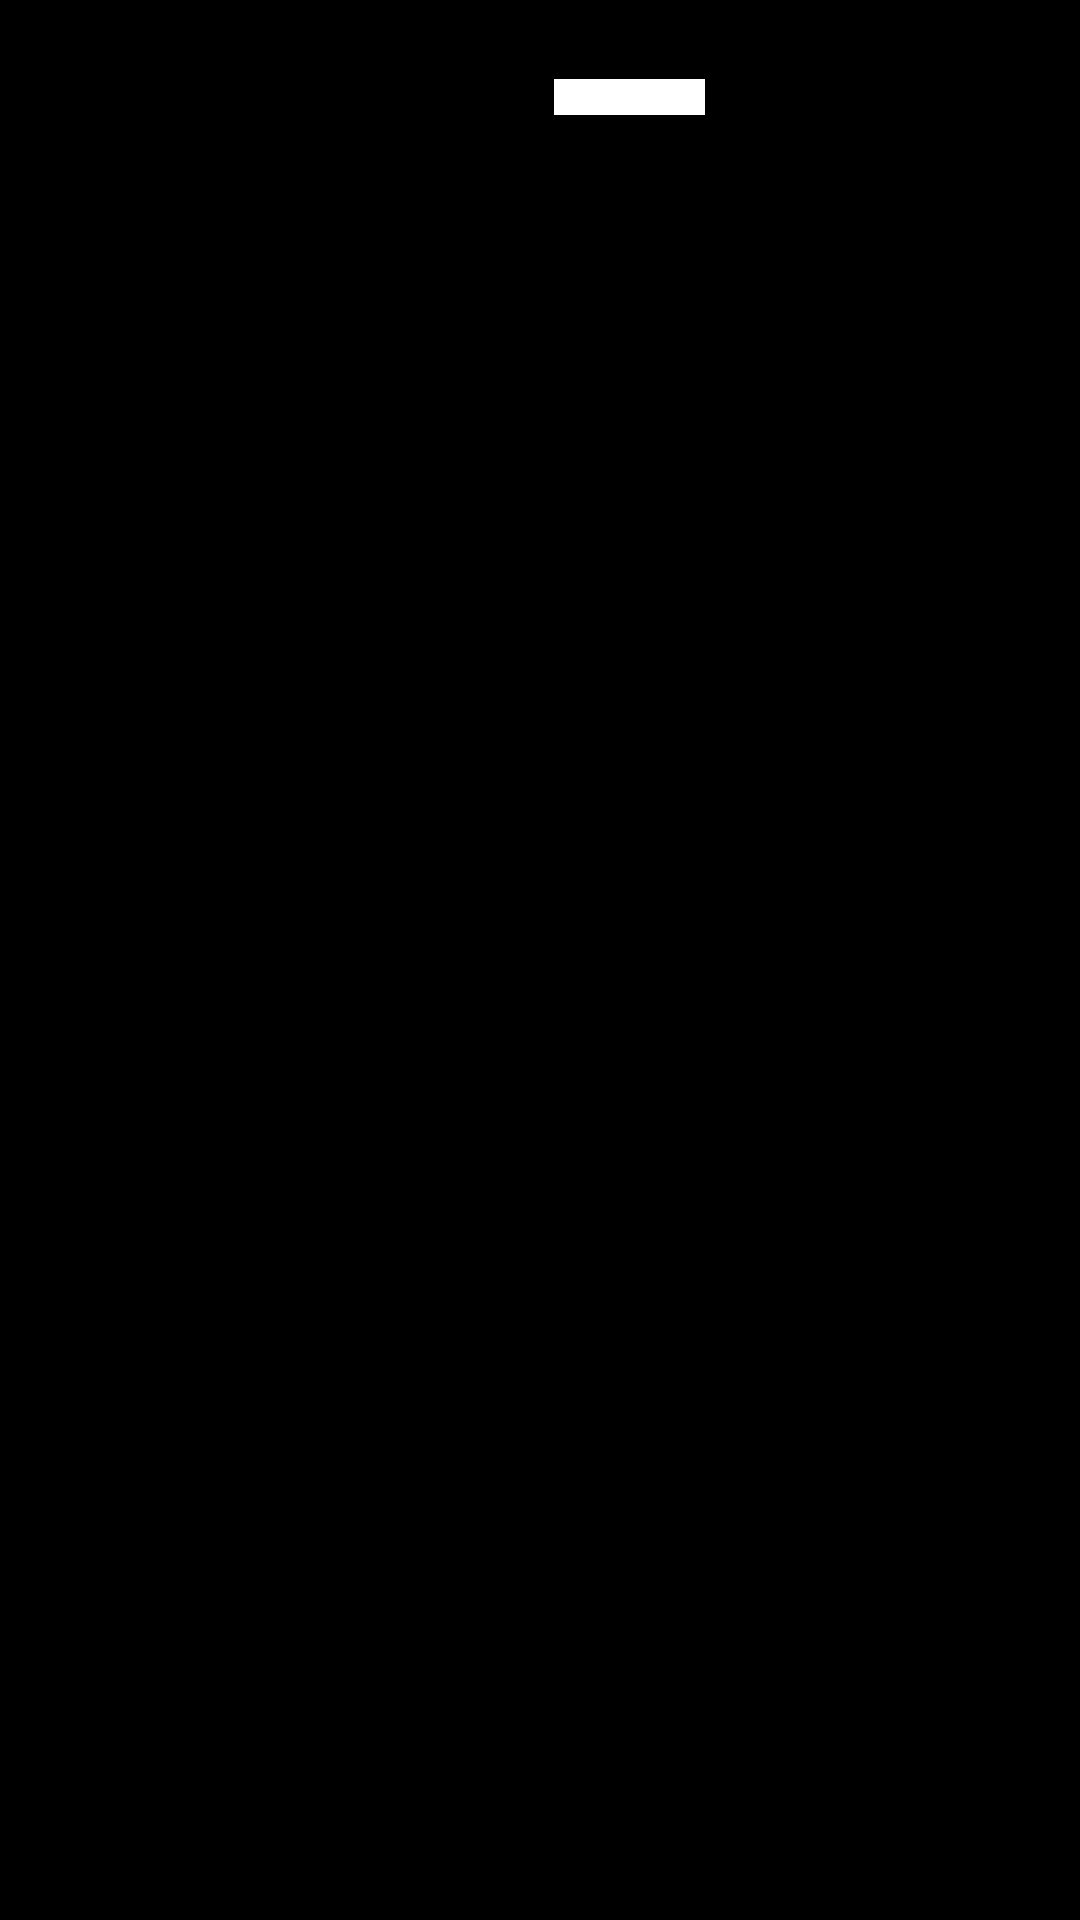
\includegraphics[scale=0.1]{img/desenvolvimento/ultrapassagemBarra/mask_head.png}
        \caption*{Fonte - Próprio Autor.}
    \end{figure}
\end{frame}


\begin{frame}{Ultrapassagem do queixo à barra - Representação da área de interesse}
    \begin{figure}[!ht]
        \centering
            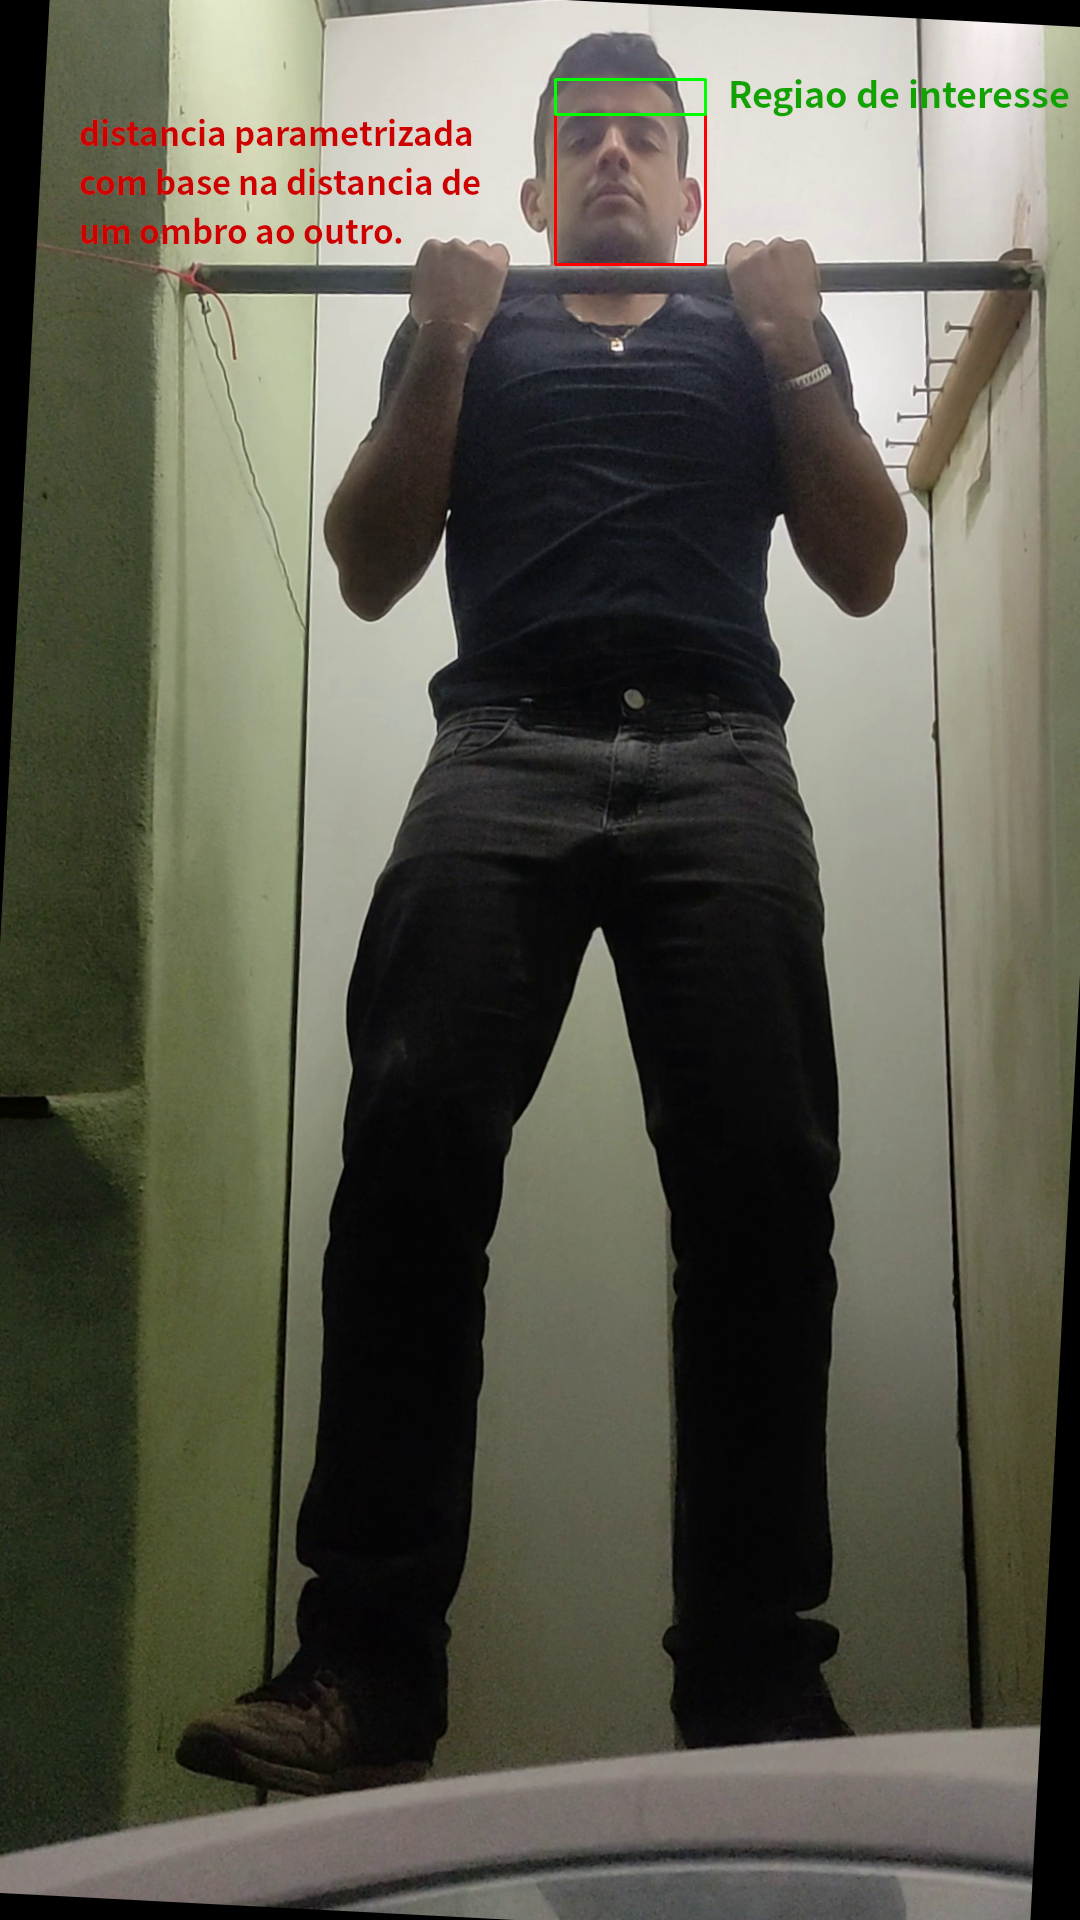
\includegraphics[scale=0.1]{img/desenvolvimento/ultrapassagemBarra/representação.png}
        \caption*{Fonte - Próprio Autor.}
    \end{figure}
\end{frame}


\begin{frame}{Ultrapassagem do queixo à barra - Imagem Segmentada}
    \begin{figure}[!ht]
        \centering
            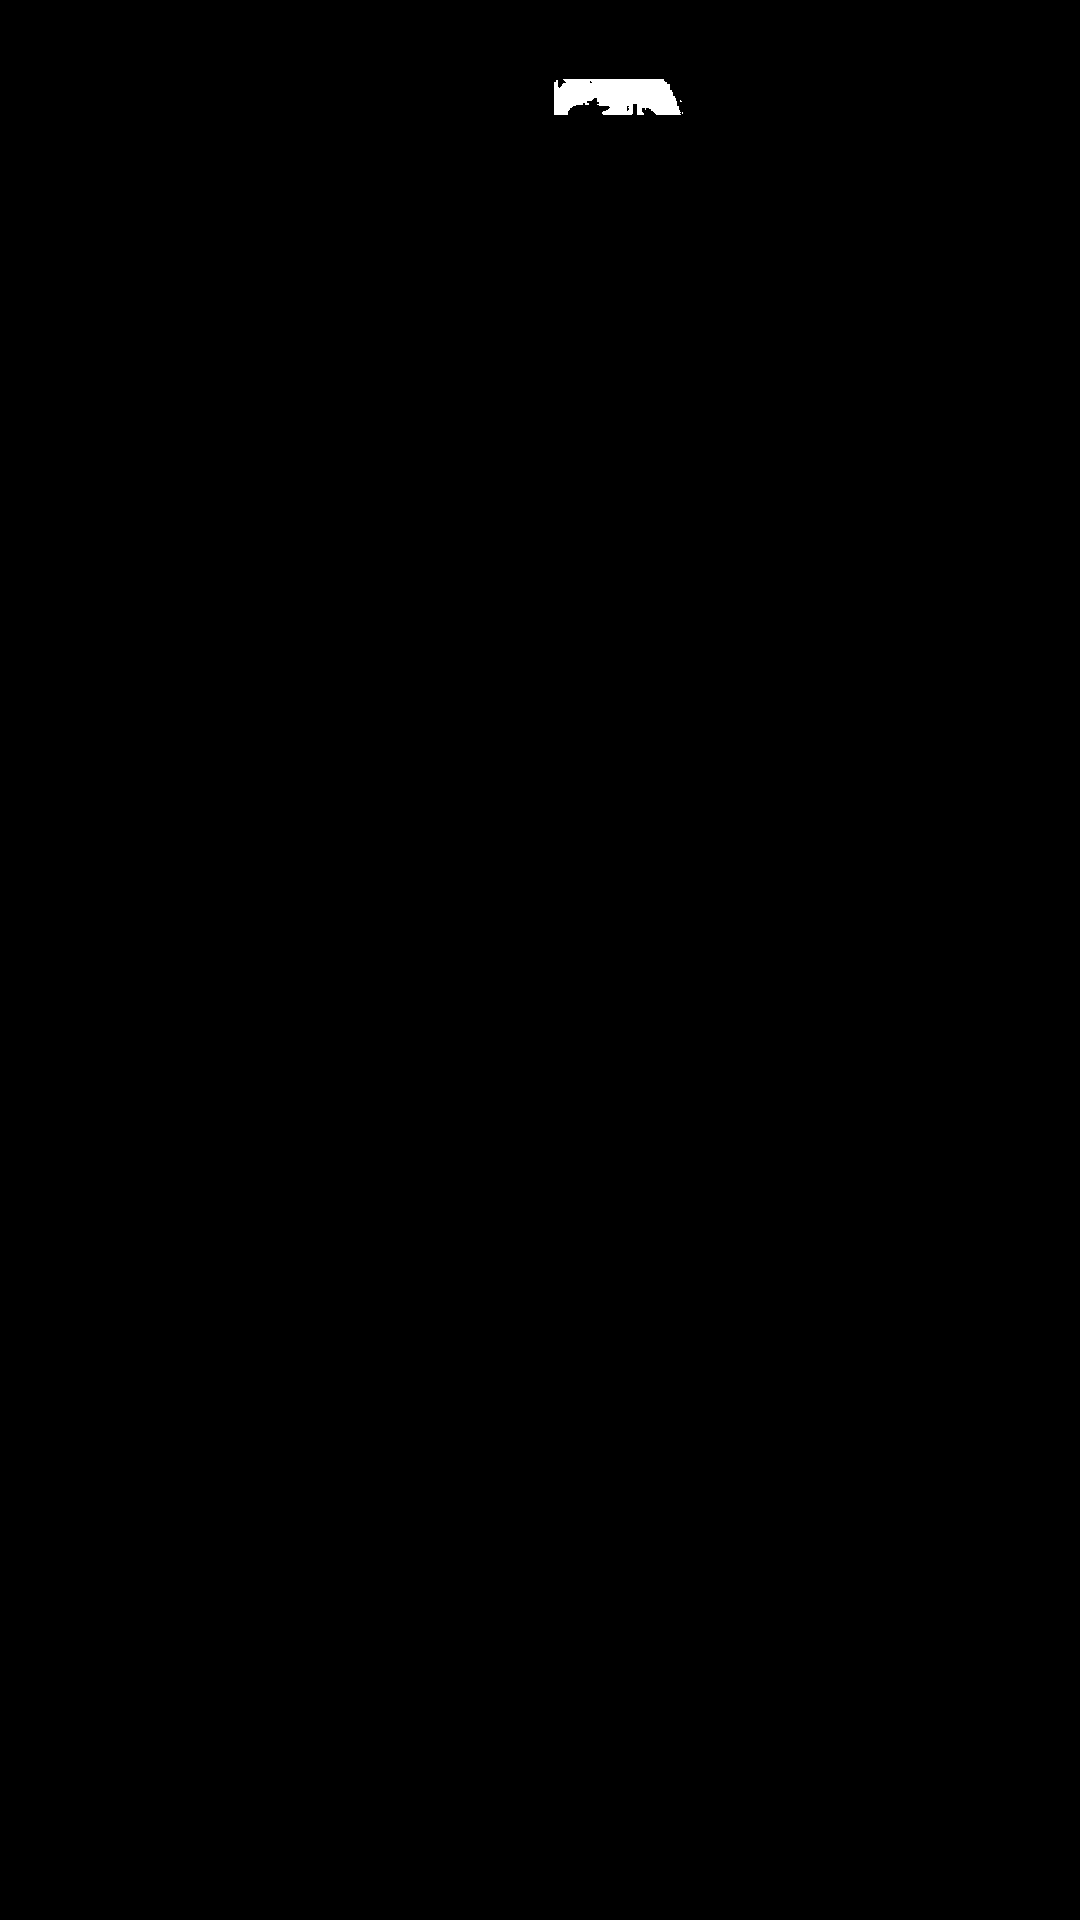
\includegraphics[scale=0.1]{img/desenvolvimento/ultrapassagemBarra/only_interesse.png}
        \caption*{Fonte - Próprio Autor.}
    \end{figure}
\end{frame}

%%%%%%%%%%%%%%%%%%%%%%%%%%%%%%%%%%%%%%%%%%%%%%%%%%%%%%%%%%%%%%%%%%%%
%%
%%                     Movimentação do quadril
%%
%%%%%%%%%%%%%%%%%%%%%%%%%%%%%%%%%%%%%%%%%%%%%%%%%%%%%%%%%%%%%%%%%%%%

\begin{frame}{Movimentação do quadril}

\begin{itemize}
        \item O movimento do quadril foi examinado de maneira semelhante à flexão e extensão
do cotovelo, no entanto, os pontos de referência utilizados foram o quadril, o joelho e o
tornozelo. 

        \item  A coxa foi considerada como o segmento de linha que se estende do quadril ao
joelho, enquanto a perna foi definida como o segmento de linha que se estende do joelho
até o tornozelo. Para avaliar a movimentação dos membros inferiores, foi analisado se o
ângulo entre os membros ou direito ou esquerdo excedia 15 graus de movimento.
    \end{itemize}
    
    
   

    
\end{frame}
